\documentclass[sigconf]{acmart}

\usepackage{syntax}
\usepackage{booktabs} % For formal tables
\usepackage{tikz}
\usetikzlibrary{arrows,shadows,positioning}
\usepackage{pgf-umlsd}
\usepackage{tikz-uml}
\usepackage{hyperref}
\usepackage{upquote}
\usepackage{listings}
\usepackage{lsthaskell}
\usepackage{xspace}
\usepackage{algorithmic}
\usepackage{longtable}
\usepackage{pgfplots}
\usepackage[titlenotnumbered, linesnumbered, ruled]{algorithm2e} % language for algorithm description
\hypersetup{
  colorlinks   = true, %Colours links instead of ugly boxes
  urlcolor     = blue, %Colour for external hyperlinks
  linkcolor    = red, %Colour of internal links
  citecolor    = green %Colour of citations
}


%%%%%%%%%%%%%%%%%%%%%%%%%%%%%%%%%%%%%%%%%%%%%%%%%%%%%%%%%%%%%
\definecolor{ltblue}{rgb}{0,0.4,0.4}
\definecolor{dkblue}{rgb}{0,0.1,0.6}
\definecolor{dkgreen}{rgb}{0,0.4,0}
\definecolor{dkviolet}{rgb}{0.3,0,0.5}
\definecolor{dkred}{rgb}{0.5,0,0}

\definecolor{lightgray}{rgb}{0.95, 0.95, 0.95}
\definecolor{darkgray}{rgb}{0.4, 0.4, 0.4}
%\definecolor{purple}{rgb}{0.65, 0.12, 0.82}
\definecolor{editorGray}{rgb}{0.95, 0.95, 0.95}
\definecolor{editorOcher}{rgb}{1, 0.5, 0} % #FF7F00 -> rgb(239, 169, 0)
\definecolor{editorGreen}{rgb}{0, 0.5, 0} % #007C00 -> rgb(0, 124, 0)
\definecolor{orange}{rgb}{1,0.45,0.13}		
\definecolor{olive}{rgb}{0.17,0.59,0.20}
\definecolor{brown}{rgb}{0.69,0.31,0.31}
\definecolor{purple}{rgb}{0.38,0.18,0.81}
\definecolor{lightblue}{rgb}{0.1,0.57,0.7}
\definecolor{lightred}{rgb}{1,0.4,0.5}
% CSS
\lstdefinelanguage{CSS}{
  keywords={color,background-image:,margin,padding,font,weight,display,position,top,left,right,bottom,list,style,border,size,white,space,min,width, transition:, transform:, transition-property, transition-duration, transition-timing-function},	
  sensitive=true,
  morecomment=[l]{//},
  morecomment=[s]{/*}{*/},
  morestring=[b]',
  morestring=[b]",
  alsoletter={:},
  alsodigit={-}
}

% JavaScript
\lstdefinelanguage{JavaScript}{
  morekeywords={typeof, new, true, false, catch, function, return, null, catch, switch, var, if, in, while, do, else, case, break, for},
  morecomment=[s]{/*}{*/},
  morecomment=[l]//,
  morestring=[b]",
  morestring=[b]'
}

\lstdefinelanguage{HTML5}{
  language=html,
  sensitive=true,	
  alsoletter={<>=-},	
  morecomment=[s]{<!-}{-->},
  morestring=[b]'
  tag=[s],
  otherkeywords={
  % General
  >,
  % Standard tags
	<!DOCTYPE,
  </html, <html, <head, <title, </title, <style, </style, <link, </head, <meta, />,
	% body
	</body, <body,
	% Divs
	</div, <div, </div>, 
	% Paragraphs
	</p, <p, </p>,
	% scripts
	</script, <script,
  % More tags...
  <canvas, /canvas>, <svg, <rect, <animateTransform, </rect>, </svg>, <video, <source, <iframe, </iframe>, </video>, <image, </image>, <header, </header, <article, </article
  },
  ndkeywords={
  % General
  =,
  % HTML attributes
  charset=, src=, id=, width=, height=, style=, type=, rel=, href=,
  % SVG attributes
  fill=, attributeName=, begin=, dur=, from=, to=, poster=, controls=, x=, y=, repeatCount=, xlink:href=,
  % properties
  margin:, padding:, background-image:, border:, top:, left:, position:, width:, height:, margin-top:, margin-bottom:, font-size:, line-height:,
	% CSS3 properties
  transform:, -moz-transform:, -webkit-transform:,
  animation:, -webkit-animation:,
  transition:,  transition-duration:, transition-property:, transition-timing-function:,
  }
}

\lstdefinelanguage{HTML5}{
  language=html,
  tagstyle=\color{blue},
  markfirstintag=true,
  sensitive=true,
  alsoletter={<>=-},	
  morecomment=[s]{<!--}{-->},
  % tag=[s],
  %% morestring=[b]'',
  morestring=[b]',
  ndkeywords={
    % General
    =,
    % HTML attributes
    id=, class= 
  }
}


\lstdefinestyle{htmlcssjs} {%
  % General design
  backgroundcolor=\color{editorGray},
  basicstyle={\scriptsize\ttfamily},   
  frame=tb,
  % line-numbers
  xleftmargin={0.75cm},
  numbers=left,
  stepnumber=1,
  firstnumber=1,
  numberfirstline=true,	
  % Code design
  identifierstyle=\color{black},
  keywordstyle=\color{blue}\bfseries,
  ndkeywordstyle=\color{editorGreen}\bfseries,
  stringstyle=\color{editorOcher}\ttfamily,
  commentstyle=\color{brown}\ttfamily,
  % Code
  language=JavaScript,
  alsolanguage=HTML5,
  alsodigit={.:;},	
  tabsize=2,
  showtabs=false,
  showspaces=false,
  showstringspaces=false,
  extendedchars=true,
  breaklines=true,
  escapechar=|c
}
%%%%%%%%%%%%%%%%%%%%%%%%%%%%%%%%%%%%%%%%%%%%%%%%%%%%%%%%%%%%%

\listfiles % used to output the versions of all files being used by the latex

\newcommand{\Server}{\emph{Server}\xspace}
\newcommand{\Client}{\emph{Client}\xspace}
\newcommand{\User}{\emph{User}\xspace}
\newcommand{\Validator}{\emph{Validator}\xspace}
\newcommand{\thenBr}{\text{then}}
\newcommand{\elseBr}{\text{else}}
\newcommand{\inFor}{\text{inFor}}
\newcommand{\inWhile}{\text{inWhile}}


% Copyright
%\setcopyright{none}
%\setcopyright{acmcopyright}
%\setcopyright{acmlicensed}
\setcopyright{rightsretained}
%\setcopyright{usgov}
%\setcopyright{usgovmixed}
%\setcopyright{cagov}
%\setcopyright{cagovmixed}


% DOI
\acmDOI{10.475/123_4}

% ISBN
\acmISBN{123-4567-24-567/08/06}

%Conference
\acmConference[ISSTA'18]{ACM SIGSOFT International Symposium on Software Testing and Analysis}{July 2018}{Amsterdam, The Netherlands} 
\acmYear{1997}
\copyrightyear{2016}

\acmPrice{15.00}


\begin{document}
\title{Search-Based Test Data Generation for JavaScript Functions with DOM}


%% \author{
%%   \alignauthor Alexander Elyasov, Wishnu Prasetya, Jurriaan Hage\\ 
%%   \affaddr{Utrecht University, The Netherlands}\\
%%   \email{\{a.elyasov,s.w.b.prasetya,j.hage\}@uu.nl}
%% }

\author{Alexander Elyasov}
\affiliation{%
  \institution{Utrecht University}
  \city{Utrecht} 
  \country{The Netherlands} 
}
\email{a.elyasov@uu.nl}

\author{Wishnu Prasetya}
\affiliation{%
  \institution{Utrecht University}
  \city{Utrecht} 
  \country{The Netherlands} 
}
\email{s.w.b.prasetya@uu.nl}

\author{Jurriaan Hage}
\affiliation{%
  \institution{Utrecht University}
  \city{Utrecht} 
  \country{The Netherlands} 
}
\email{j.hage@uu.nl}


\begin{abstract}
This paper provides a sample of a \LaTeX\ document which conforms,
somewhat loosely, to the formatting guidelines for
ACM SIG Proceedings.\footnote{This is an abstract footnote}
\end{abstract}

%
% The code below should be generated by the tool at
% http://dl.acm.org/ccs.cfm
% Please copy and paste the code instead of the example below. 
%
\begin{CCSXML}
TODO 
\end{CCSXML}

\ccsdesc[500]{Computer systems organization~Embedded systems}
\ccsdesc[300]{Computer systems organization~Redundancy}
\ccsdesc{Computer systems organization~Robotics}
\ccsdesc[100]{Networks~Network reliability}


\keywords{ACM proceedings, \LaTeX, text tagging}


\maketitle


\section{Introduction}
\label{sec.intro}
Recent empirical study of client-side JavaScript bugs~\cite{frolin:TSE16} has shown that 68\% of faults are DOM related.

Another empirical work~\cite{richards2010analysis}.

%% --------------------------------------------------------------------
\section{Motivating Example}
\label{sec.example}
%% --------------------------------------------------------------------

\begin{figure}[t]
  \begin{lstlisting}[style=htmlcssjs,language=JavaScript]
/*t dom */
function isGameFinished() {
  var obj = document.getElementById('sudoku'); |c \label{isGameFinished.getSudoku} |c
  var subDivs = obj.getElementsByTagName('DIV'); |c \label{isGameFinished.getDivs} |c
  var allOk = true;
  for (var no = 0; no < subDivs.length; no++) { |c \label{isGameFinished.inFor.begin} |c
    if (subDivs[no].className.indexOf('sudokuSquare') >= 0 |c \label{isGameFinished.if1.begin} |c 
        && !subDivs[no].style.backgroundColor) { 
      var spans = subDivs[no].getElementsByTagName('SPAN');
      if (spans[0].innerHTML != spans[1].innerHTML) { |c \label{isGameFinished.if2.begin} |c
        allOk = false; |c \label{isGameFinished.unfinished} |c
        break;
      } |c \label{isGameFinished.if2.end} |c
    } |c \label{isGameFinished.if1.end} |c
  } |c \label{isGameFinished.inFor.end} |c
  if (allOk) { |c \label{isGameFinished.if3.begin} |c 
    console.log('Congratulations! You did it'); |c \label{isGameFinished.finished} |c
  } |c \label{isGameFinished.if3.end} |c
}
\end{lstlisting}
  \caption{JS function \texttt{isGameFinished.js} from sudoku}
  \label{code.newGame}
\end{figure}

\begin{figure}[t]
  \begin{lstlisting}[style=htmlcssjs,language=JavaScript]
function isGameFinished() {
  trace.push(2);
  var obj = document.getElementById("sudoku");
  trace.push(3);
  var subDivs = obj.getElementsByTagName("DIV");
  trace.push(4);
  var allOk = true;
  loopMap[5] = function () {
    var no = 0;
    if (subDivs.length || subDivs.length == 0) {
      return Math.abs(no - subDivs.length);
    }
    return 1;
  }();
  for (var no = 0; no < subDivs.length; no++) {
    trace.push(5);
    trace.push(6);
    trace.push(7);
    if (subDivs[no].className.indexOf("sudokuSquare") >= 0 &&
        !subDivs[no].style.backgroundColor) {
      trace.push(8);
      branchDistance.push({ 
        label: 7, 
        distance: Math.min(
          abs(subDivs[no].className.indexOf("sudokuSquare"), 0) + _K_,
          absZero(subDivs[no].style.backgroundColor))
      });
      trace.push(9);
      var spans = subDivs[no].getElementsByTagName("SPAN");
      trace.push(10);
      if (spans[0].innerHTML != spans[1].innerHTML) {
      trace.push(11);
      branchDistance.push({
        label: 10,
        distance: abs(spans[0].innerHTML, spans[1].innerHTML)
      });
      trace.push(12);
      allOk = false;
      break;
      } else {
        trace.push(14);
        branchDistance.push({label: 10,distance: _K_});
      }
    } else {
      trace.push(15);
      branchDistance.push({
        label: 7,
        distance: abs(subDivs[no].className.indexOf("sudokuSquare"), 0) +
                  absNegZero(subDivs[no].style.backgroundColor)
      });
    }
  }
  trace.push(5);
  trace.push(16);
  if (allOk) {
    trace.push(17);
    branchDistance.push({label: 16, distance: absNegZero(allOk)});
    trace.push(18);
    console.log("Congratulations! You did it");
  } else {
    trace.push(19);
    branchDistance.push({label: 16 ,distance: absZero(allOk)});
  }
  trace.push(-1);
}
\end{lstlisting}
  \caption{Instrumented version of the function \texttt{isGameFinished.js} }
  \label{code.isGameFinished.instr}
\end{figure}

\begin{figure}[t]
  \begin{lstlisting}[style=htmlcssjs, language=HTML5]
<!-- T1 covers: (6,15), (16,17) -->
<html>
  <body>
    <div id='sudoku'></div>
</body>
</html>

<!-- T2 covers: (6,7), (7,14), (16,17) -->
<html>
  <body>
    <div id='sudoku'>
      <div></div>
    </div>
  </body>
</html>

<!-- T3 covers: (6,7), (7,9), (10,13), (16,17) -->
<html>
  <body>
    <div id='sudoku'>
      <div class='sudokuSquare'>
        <span></span>
        <span></span>
      </div>
    </div>
  </body>
</html>

<!-- T4 covers: (6,7), (7,9), (10,11), (16,18) -->
<html>
  <body>
    <div id='sudoku'>
      <div class='sudokuSquare'>
        <span></span>
        <span>TEST</span>
      </div>
    </div>
  </body>
</html>
  \end{lstlisting}
  \caption{Input DOM arguments for \texttt{isGameFinished.js}}
  \label{fig.isGameFinished.tests}
\end{figure}

Let us consider JS function \texttt{isGameFinished} in Figure~\ref{code.newGame} taken from the web application game \emph{sudoku}~\ref{ref.sudoku}. This function checks if a sudoku solution entered by the user is valid. First, it finds the game field element (line~\ref{isGameFinished.getSudoku}), retrieves all child divs (line~\ref{isGameFinished.getDivs}), and iterates over that collection. Each div element which corresponds to a sudoku input square (line~\ref{isGameFinished.if1.begin}) consists of two span elements. One contains a user input, and another one, which is hidden at the moment, stores the expected value for the sudoku square. Once, it finds a square where two values are not equal (line~\ref{isGameFinished.if2.begin}) to each other, the game is considered unfinished (line~\ref{isGameFinished.unfinished}) and finished otherwise (line~\ref{isGameFinished.finished}).

Suppose now that we would like to (unit) test this function in isolation to the rest of the application source code. We aim to maximize branch coverage as a common testing criteria~\cite{why.this.common}. That is for each individual branch of the function under test (FUT) \texttt{isGameFinished}, we have to construct a test input which passes the branch and normally exists the function. JS function has \emph{explicit} input arguments (none is our case), but it can also has \emph{implicit} arguments such as DOM state. As assume that DOM is the only global JS object that can be referred from the body of FUT. So in order to test our function we have to construct appropriate DOM objects as test inputs.   

%Our program has the following branches: $(6,15)$, $(6,7)$, $(7,9)$, $(7,14)$, $(10,11)$, $(10,13)$, $(16,17)$, $(16,18)$. Four tests in 

Figure~\ref{fig.isGameFinished.tests} presents four tests that together provide full coverage of the FUT. Let us look at how to construct the test that covers branch $(10,11)$. Line~\ref{isGameFinished.getSudoku} expects DOM to have an element with the id \textquotesingle\texttt{sudoku}\textquotesingle. In order to enter the for-loop on line~{isGameFinished.inFor.begin}, this element should have at least one child of the type $div$. The condition of the first $if$ (line~\ref{isGameFinished.if1.begin}) requires the div to be of the class \textquotesingle\texttt{sudokuSquare}\textquotesingle and have no background color. The last if-condition (line~\ref{isGameFinished.if2.begin}) expects that the div has two \emph{span} elements whose \emph{innerHtml} values are not equal. $T4$ in Figure~\ref{fig.isGameFinished.tests} shows a concrete example of DOM that meets all the conditions above. 

As we have just seen even for such a relatively simple example, the construction of the test input is a far from trivial procedure because it requires deep understanding the program's semantics. In practice, web developers often have to deal with the gazillion of the JS frameworks and libraries freely available on the GitHub. This code is commonly untested and poorly documented. At the same time, unit testing is the most fundamental and easiest to provide level of testing. It greatly saves developers from the unexpected regression and creates a safety belt around the application.

%% --------------------------------------------------------------------
\section{Test Generation Framework}
\label{sec.framework}
%% --------------------------------------------------------------------

\begin{figure}[t!]
  \centering 
  \begin{sequencediagram}[font=\footnotesize]

    \renewcommand\unitfactor{0.5}
    \newinst{user}{\textbf{User}}
    \newinst{server}{\textbf{Server}}
    \newinst[1]{validator}{\textbf{Validator}}
    \newinst{client}{\textbf{Client}}
    
    \begin{call}{user}{fun.js + config}{server}{\textbf{end}}
      \begin{call}{server}{Initialize(fun.js)}{server}{(cfg, branches, cinfo, ifun, sig)}
      \end{call}
      
      \begin{call}{server}{POST /init \{ifun, sig\}}{client}{status}
      \end{call}
      
      \begin{call}{server}{Select(branches)}{user}{$\text{branches}'$}       
      \end{call}
      
      \begin{sdblock}{\textbf{Genetic Loop}}{\hspace{2mm}$\text{branch} \in \text{branches}'$}
        \begin{sdblock}{\textbf{Random Loop}}{errors > 0}
          \begin{call}{server}{pop = Random(cinfo, config)}{validator}{errors}
          \end{call}
          \prelevel
        \end{sdblock}
        
        \begin{sdblock}{\textbf{Fitness Loop}}{(fitness $\neq$ 0) $\vee$ gen.limit}

          \begin{sdblock}{\textbf{Evaluation Loop}}{p $\in$ pop}
            \begin{call}{server}{POST /genetic \{p\}}{client}{response = ifun(p: sig)}
            \end{call}
            
            \begin{callself}{server}{Evaluate(branch, cfg, response)}{fitness}
            \end{callself}
            \prelevel
          \end{sdblock}
          
          \begin{sdblock}{\textbf{Crossover Loop}}{errors > 0}
            \begin{call}{server}{cross = Crossover(cinfo, pop)}{validator}{errors}
            \end{call}
            \prelevel
          \end{sdblock}

          \begin{sdblock}{\textbf{Mutation Loop}}{errors > 0}
            \begin{call}{server}{mut = Mutation(cinfo, pop)}{validator}{errors}
            \end{call}
            \prelevel
          \end{sdblock}
         
          \begin{callself}{server}{pop = cross $\cup$ mut}{pop}
          \end{callself}
          \prelevel
        \end{sdblock}
        \mess{server}{best fitness}{user}
        
      \end{sdblock}
    \end{call}
  \end{sequencediagram}
  \caption{Architecture of the test framework}
  \label{fig.framework.architect} 
\end{figure}

Given JS function $f$ and a set of branches $\mathbb{B}_f$, the ultimate goal of the testing framework is to find input arguments for $f$ that cover all branches from $B_f$. We implemented such a framework as a client-server application which uses under the hood genetic test generation engine. The general workflow of the framework is depicted as a sequence diagram in Figure~\ref{fig.framework.architect}. The diagram consists of the four interacting components \User, \Server, \Validator, and \Client. \Server is the key component of the whole framework. It is responsible for the \emph{Initialization Phase} and test data generation in the \emph{Genetic Phase}. Both phases will be covered in details in Section~\ref{sub.sec.init.phase} and \ref{sub.sec.genetic.phase} respectively. Each newly constructed HTML document has to be processed by the \Validator\footnote{\url{https://validator.w3.org/nu/}} which checks its syntactical correctness and reports back the set of identified errors. \Server rejects the document if any errors were revealed and repeats the current step until the generated document has no errors anymore. \Client is a \emph{Node.js}\footnote{\url{https://nodejs.org/en/}} application that is mainly responsible for the execution of the JS code. We use the \emph{jsdom}\footnote{\url{https://github.com/tmpvar/jsdom}} library to model the virtual DOM and simulate native browser API calls.   

Let us give a closer look at the sequence of interactions in Figure~\ref{fig.framework.architect}. As an input to our testing framework, \User has to provide the JS file \emph{fun.js} that contains the function under test (FUT) \emph{fun} annotated with the type signature. Additionally, \User specifies a configuration file \emph{config} that defines various parameters for random data generation, genetic phase, logging etc. Experimentally, we have found an optimal set of input configurations that was used across all the experimental subjects in Section~\ref{sec.evaluation}. The received data is processed by \Server during the \emph{Initialization Phase}. At the end of it we get the following information back: the control flow graph (\emph{cfg}) of \emph{fun}, the list of its branches (\emph{branches}), the \emph{fun}'s  constant (\emph{cinfo}) info, the instrumented version \emph{ifun} of \emph{fun}, and the \emph{fun}'s signature (\emph{sig}). \Server sends a \texttt{POST} request to the \Client to store there \emph{ifun} and \emph{sig}. Depending on the chosen execution mode, the \Server either asks the \User to select the target branch or covers all branches one by one in a fixed order. For each branch our framework enters the \emph{Genetic Loop (Phase)}. Inside of this phase, the framework starts with a randomly generated population (\emph{Random Loop}), and continues to evolve the population (\emph{Fitness Loop}) until either a perfect entity is found or a certain termination criteria is achieved, e.g. the limit of generation attempts is reached. Each candidate in the population has to be evaluated in \emph{Evaluation Loop} by \Client. It matches the candidate $p$ according the known type signature \emph{sig} and invokes the instrumented JS function \emph{ifun(p)}. The execution trace along with some collected information are sent back to the \Server, where the final fitness value is computed. The new population is constructed by combining the results of the \emph{Crossover} and \emph{Mutation Loops}. If an HTML document is produced during one the genetic phases, it has to be approved by the \Validator first. At the end of the \emph{Fitness Loop} the candidate with the ``best'' fitness value is reported back to the \User. Once all branches are exercised, the algorithm reaches the end. In the follow up two sections we elaborate on the details of each individual component of our test generation framework.

\subsection{Initialization Phase}
\label{sub.sec.init.phase}

\begin{algorithm}[t!]
  \caption{Initialization Phase}
  \label{alg.init}
  \algsetup{linenosize=\tiny}
  \scriptsize
  \DontPrintSemicolon
  \SetAlgoVlined
  \SetKwInOut{Input}{Input}
  \SetKwInOut{Output}{Output}
  \SetKwInOut{Require}{Require}
  \SetKwProg{Fn}{Function}{}{}
  \Input{JS file $fun.js$ with FUT and type annotation }
  \Output{Tuple $(cfg, branches, cinfo, ifun, sig)$}
  \Fn{$Initialize(fun.js)$}{
 
    $(ast, sig) \longleftarrow ParseFuncAndSig(fun.js)$\label{alg.init.parse.fun.sig}\;
    $cinfo \longleftarrow GetConstantInfo(ast)$\label{alg.init.collect.info}\;
    $nast \longleftarrow NormalizeAST(ast)$\label{alg.init.transform.ast}\;
    $ifun \longleftarrow Instrument(nast)$\label{alg.init.instr}\;
    $cfg \longleftarrow BuildCFG(nast)$\label{alg.init.build.cfg}\;
    $branches \longleftarrow GetBranches(cfg)$\label{alg.init.get.branches}\;
    \Return{$(cfg, branches, cinfo, ifun, sig)$}
    }
\end{algorithm}

During the \emph{Initialization Phase} we analyze FUN and collect data necessary for the consecutive genetic testing phase. The main steps of the initialization are illustrated in Algorithm~\ref{alg.init}. Given a FUT \emph{fun.js} as an input, we parse the function and its type signature in line~\ref{alg.init.parse.fun.sig}. In order to maximize the chances of generating the fittest candidate in the genetic phase, we perform a static analysis of the FUT with the purpose to collect constant info in line~\ref{alg.init.collect.info}. Such constants include string and numeric literals as well as the arguments to the following DOM API methods:
\begin{itemize}
\item \texttt{getElementsByTagName}
\item \texttt{getElementById}
\item \texttt{getElementsByClassName}
\item \texttt{getElementsByName}
\end{itemize}
which respectively signify the reference to the \emph{tags}, \emph{ids}, \emph{classes} and \emph{names} used in the FUT. Next step is normalizing the FUT before applying any instrumentation (line~\ref{alg.init.transform.ast}), e.g. we need to transform \emph{if-then} branches into \emph{if-then-else}. We need to instrument the FUT (line~\ref{alg.init.instr}) in order be able to collect the run-time data such as the execution trace, the approach level, the branch and loop distances, and the constants. Upon the $ifun$ execution this information is gathered and fed back to the fitness evaluation procedure. The last two steps are to construct the control-flow graph (line~\ref{alg.init.build.cfg}) and identify all branches of the FUT (line~\ref{alg.init.get.branches}).

\subsubsection{Supported Types}
\label{sub.sec.sup.types}

\begin{figure}[t]
\setlength{\grammarparsep}{3pt}
\small
\begin{grammar}

<JS Type Annotation> ::= /*t <Signature> */

<Signature> ::= <DOM> : <Type Signature> | <Type Signature>

<DOM> ::= \texttt{dom}

<Type Signature> ::= <Type> | <Type> : <Type Signature>

<Type> ::= <Void Type> | <Primitive Type> | <Array Type>

<Primitive Type> ::= \texttt{bool} | \texttt{int} | \texttt{float} | \texttt{string}

<Array Type> ::= [ <Primitive Type> ] | [ <Array Type> ]
\end{grammar}
\caption{Grammar of supported JS type annotations}
\label{fig.js.type.annot}
\end{figure}

The grammar of JS type annotations supported by our test generation framework is shown in Figure~\ref{fig.js.type.annot}. Each type annotation is a signature surrounded with a specialized JS type comment (\texttt{/*t...*/}). We distinguish two between kinds of signatures those who refer to the global DOM and ``ordinary'' JS type signatures. Functions with a DOM signature expect a \texttt{dom} argument being passed as the first implicit parameter to the function call. Ordinary JS signature is a non-zero sequence of JS types. The type can be \emph{Void}, \emph{Primitive} (\texttt{bool}, \texttt{int}, \texttt{float}, \texttt{string}) or \emph{Array} (recursive homogeneous array type).  


\subsection{Genetic Phase}
\label{sub.sec.genetic.phase}

\begin{algorithm}[!t]
  \caption{Genetic Phase}
  \label{alg.gen}
  \algsetup{linenosize=\tiny}
  \scriptsize
  \DontPrintSemicolon
  \SetAlgoVlined
  \SetKwInOut{Input}{Input}
  \SetKwInOut{Output}{Output}
  \SetKwInOut{Require}{Require}
  \SetKwProg{Fn}{Function}{}{}
  \Input{
    $config$ is a GA configuration file\\
    $b_n$ is a target branch of FUT\\
    $(cfg, branches, cinfo, ifun, sig)$ output of Algorithm~\ref{alg.init}
  }
  \Output{
     $(f^*, p^*)$ the best population candidate and its fitness score
  }
  \Fn{$Genetic(b_n, cfg, cinfo, config, ifun, sig)$}{
    $(size_P, size_A, size_G, rate_C, rate_M,size_{H}) \longleftarrow Read(config)$\label{alg.gen.read.config}\;
    $target \longleftarrow b_n$\label{alg.gen.init.target}\; 
    $i \longleftarrow 0 $\label{alg.gen.iter.count}\;
    \Repeat{$\neg historyConverged \vee (i > size_G)$}{\label{alg.gen.converged.loop.begin}
      $archive \longleftarrow \emptyset$\label{alg.gen.init.archive}\; 
      $history \longleftarrow \emptyset$\label{alg.gen.init.history}\; 
      $pop \longleftarrow Random(cinfo, size_P)$\label{alg.gen.random.gen}\;
      \Repeat{$isPerfect(f^*) \vee historyConverged \vee (i > size_G)$}{\label{alg.gen.loop.begin}
        $scoredPop \longleftarrow \emptyset$\;
        $history \longleftarrow history \cup archive$\;
        \ForAll{$p \in pop$}{\label{alg.gen.eval.begin}
          $args \longleftarrow CoerceArguments(p, sig)$\label{alg.gen.make.args}\;
          $(tr, d_B, d_L, dyncinfo) \longleftarrow ifun(args)$\label{alg.gen.call.ifun}\;
          $f \longleftarrow Score(target, cfg, tr, d_B, d_L)$\label{alg.gen.eval}\;
          $cinfo \longleftarrow cinfo \cup dyncinfo$\label{alg.gen.eval.end}\;
          $scoredPop \longleftarrow (f, p) \cup scoredPop$\;
        }
        $combo \longleftarrow scoredPop \cup archive$\label{alg.gen.get.combo}\;
        $cross \longleftarrow Crossover(combo, rate_C)$\label{alg.gen.cross}\;
        $mut \longleftarrow Mutation(combo, cinfo, rate_M)$\label{alg.gen.mut}\;
        $pop \longleftarrow cross \cup mut$\label{alg.gen.new.pop}\;
        $archive \longleftarrow SortArchive(combo, size_A)$\label{alg.gen.new.archive}\;
        $(f^*, p^*) \longleftarrow head(archive)$\label{alg.gen.archive.head}\;
        $i \longleftarrow i + 1$\;
        $historyConverged \longleftarrow hasConverged(history, size_H)$\label{alg.gen.has.converged}\;
      }\label{alg.gen.loop.end}
      $target \longleftarrow NewTarget(branches, b_n)$\label{alg.gen.new.target}\;
    }\label{alg.gen.converged.loop.end}
    \Return{$(f^*, p^*)$}\label{alg.gen.return} 
  }
\end{algorithm} 

The heart of our test data generation framework is in the \emph{Genetic Phase}. The main workflow of the underlying genetic algorithm (GA) is, though, being fairly standard~\cite{poli2008field} but has been extended with the concept of \emph{archive convergence} (Algorithm~\ref{alg.gen}). We get as an input a configuration file \emph{config}, a target branch $b_n$ of the FUT (which we would like to cover), and the tuple of parameters computed by Algorithm~\ref{alg.init}. The output consists of the ``best'' fitness score $f^*$ achieved on the population candidate $p^*$.

First, we read the \emph{config} file (line~\ref{alg.gen.read.config}) and retrieve the following GA configuration parameters: 
%% \begin{itemize}
%% \item $size_P$ is the size of the genetic population
%% \item $size_A$ is the size of the genetic archive
%% \item $size_G$ is the total number of the genetic iterations
%% \item $rate_C$ is a crossover rate
%% \item $rate_M$ is a mutation rate
%% \item $size_H$ is a history window size
%% \end{itemize}
a population size  ($size_P$), an archive size ($size_A$), the number of generations ($size_G$), crossover ($rate_C$) and mutation ($rate_M$) rates respectively, and a history window size ($size_H$). We set the initial target to $b_n$ (line~\ref{alg.gen.init.target}) and the iteration counter $i$ to 0 (line~\ref{alg.gen.iter.count}). Until the history of archives has not converged or the limit of the generations has not been reached, we are initializing the genetic search of the target branch (lines~\ref{alg.gen.converged.loop.begin}-\ref{alg.gen.converged.loop.end}). An \emph{archive} stores the most fitted population candidates observed so far. It is empty in the beginning of the evolution (line~\ref{alg.gen.arch.init}) as well as the history of archives \emph{history} (line~\ref{alg.gen.init.history}). The first population of $size_P$ elements is randomly generated out of the constants taken from \emph{cinfo} (line~\ref{alg.gen.random.gen}). Then, in loop lines~\ref{alg.gen.loop.begin}-\ref{alg.gen.loop.end}, this population is evolved until either the perfect candidate is found or the history of archives is converged or the generation limit $size_G$ is reached. But the first step in this loop is scoring the current population~\ref{alg.gen.eval.begin}-\ref{alg.gen.eval.end}. Each candidate of the population represents a concrete argument list of the FUT so it has to be coerced with respect to the type signature $sig$ (line~\ref{alg.gen.make.args}). After calling the instrumented function \emph{ifun} on $args$ (line~\ref{alg.gen.call.ifun}), we get 4-tuple consisting of an execution trace ($tr$), the sets of branch ($d_B$) and loop distances ($d_L$), and dynamic constant info (\emph{dyncinfo}) collected at the run-time. The next step is actually scoring the fitness value for the given population candidate (line~\ref{alg.gen.eval}). Collected constants \emph{dyncinfo} are merged with existing constant pool (line~\ref{alg.gen.eval.end}). Eventually, the scored population is combined with the archive (line~\ref{alg.gen.get.combo}) and it is used for the crossover (line~\ref{alg.gen.cross}) and mutation steps (line~\ref{alg.gen.mut}). The rates specify the proportion in with two operation contribute the formation of the new population (line~\ref{alg.gen.new.pop}). The scored population together with the current archive are sorted by the fitness value, and the best $size_A$ elements form a new archive (line~\ref{alg.gen.new.archive}). The element at the top of the archive is the fittest candidate (line~\ref{alg.gen.archive.head}). The fitness value of that element defines if a perfect candidate is found (line~\ref{alg.gen.loop.end}). Eventually, the tuple $(f^*, p^*)$ is returned by the algorithm (line~\ref{alg.gen.return}).

In some cases, when we do get enough guidance from the fitness function, the genetic algorithm converges to a local minimum~\cite{ga.flag.problem.or.survey}. For example, if one branch is dominated by another, the coverage of the former branch depends on the coverage of the latter. Unless this relation is captured by the branch condition on the former branch, the respective fitness function does not reflect on the branch dependency. In this situation, we find ourselves being trapped on a flat space, with a small unreliable chance to escape. In order to overcome this problem, we propose a novel --- to the best of our knowledge --- solution based on the idea of \emph{archive convergence}. If during a certain history window, the fitness values of the respective archives converge to a fixed point, we restart the genetic search and redefine the search target. At the end of the evolution loop (line~\ref{alg.gen.has.converged}), we compute the convergence condition of the fitness values in the first $size_H$ archives taken from the history. If the fitness has converged (line~\ref{alg.gen.loop.end}), the genetic algorithm is restarted with a new target. It consists of the original branch $b_n$ prefixed with a branch $b \in branches$ which our branch depends on (line~\ref{alg.gen.new.target}). Every time genetic search converges, we produce a new partial path by eventually covering all possible executions leading to $b_n$. In practice, we limit this process by the target of length two.

In the rest of this section, we elaborate on the technical details of the genetic algorithm such as random generation in Section~\ref{sub.sub.sec.random.html}, mutation and crossover in Section~\ref{sub.sub.sec.genetic.oper}, and fitness function in Section~\ref{sub.sub.sec.fitness.fun}. Our primary focus in those sections will be on the generation and transformation of the HTML documents. Table~\ref{} descries how similar operations are implemented for primitive and array JS types. 

\begin{table}
  \caption{Genetic Operation for JS types}
  \label{tbl.gen.oper.js.types}
    \footnotesize
  \begin{tabular}{p{1cm}|p{5mm}|p{6cm}}
    \toprule
    \textbf{Operation} & \textbf{Type} & \textbf{Description} \\
    \midrule
    Random & Bool & choose at random \{\texttt{true}, \texttt{false}\} \\
    Random & Int  & with 80\% probability choose an integer from [-10, 10], or with 20\% from integer constants\\
    Random & Float & with 80\% probability choose an float from [-10.0, 10.0], or with 20\% from float constants\\
    Random & String & with 80\% probability make a random string up to length five composed characters \texttt{[a-zA-Z0-9]}, or with 20\% from string constants\\
    Random & Array & make a random array of a respective type upto length five\\
    \midrule
    Crossover & Bool   & pick at random one out of two given boolean \\
    Crossover & Int    & pick at random one out of two given integers\\
    Crossover & Float  & pick at random one out of two given floats\\
    Crossover & String & choose independently crossover point for each string, swap ends, and pick result at random\\
    Crossover & Array & similar crossover operator as for strings\\
    \midrule
    Mutation & Bool & Flip the boolean constant\\
    Mutation & Int  & Generate a new integer value, on increase (decrease) by 1 or 10 the given one\\
    Mutation & Float  & Generate a new float value, on increase (decrease) by 0.1, 1 or 10 the given one\\
    Mutation & String & Generate an new string values, remove a random character in a string, or replace a successor (predecessor) a random character\\
    Mutation & Array & Mutate a random element in array according to its type\\
    \bottomrule
  \end{tabular}
\end{table}

\subsubsection{Random HTML Generation}
\label{sub.sub.sec.random.html}

We want to generate HTML as it is specified by WHATWG\footnote{\url{https://html.spec.whatwg.org}}. HTML is an XML-family markup language that uses special tags and attributes to describe document structures on the Web. Recent HTML5 standard defines more than hundred of tags and attributes which both have to comply with extremely complex logic to constitute a syntactically valid HTML. Browsers are usually tolerant to syntactic errors in HTML. They will silently fix them and display the page anyway.

In order to support the variability of HTML content, we have developed an eDSL that prescribes the generation of syntactically valid HTML. This was a challenge on its own because, as we have mentioned early, the complexity of HTML and lack of formal specification. Our language is inspired by QuickCheck~\cite{claessen2011quickcheck} and essentially employs the library\footnote{\url{https://hackage.haskell.org/package/QuickCheck}} to define an \texttt{Arbitrary} instance for the \texttt{Html} data type. With some technical details left out for the sake of simplicity, Figure~\ref{fig.html.arb.def} highlights that definition. Data type \texttt{HtmlState} (lines~\ref{ref.HtmlState.begin}--\ref{ref.HtmlState.end}) describes the internal state of \texttt{Html} during generation. The state is composed of the following components:
\begin{itemize}
\item \texttt{depth} and \texttt{degree} specify maximum depth and node degree of HTML respectively
\item \texttt{ctx} is the current value of the HTML content model stack 
\item \texttt{tagFreq} provides statistical information about the frequency of tags in HTML
\item \texttt{tags}, \texttt{ids} and \texttt{classes} are predefined sets of HTML elements which are given preference in the generation process.  
\end{itemize}
Combined with the random generation monad \texttt{Gen}, this state is wrapped into a state monad transformer~\cite{jones1995functional} (line~\ref{ref.GenState}) which returns the randomly generated \texttt{Html} (line~\ref{ref.GenHtmlState}). Each HTML tag should be defined as a value of type \texttt{GenHtmlState}. Lines~\ref{ref.generateHTML.begin}--\ref{ref.generateHTML.end} show an example of content generation for the \texttt{<html>} tag. According to its specification\footnote{\url{https://html.spec.whatwg.org/multipage/semantics.html\#the-html-element}}, the tag is composed of the \texttt{<head>} tag followed by the \texttt{<body>} tag. First, we store the state of HTML generation and retrieve the current the depth (lines~\ref{ref.generateHTML.getState} and \ref{ref.generateHTML.getDepth} respectively). Then, if depth is equal to zero, we just return some string constant (line~\ref{ref.generateHTML.returnString}). Otherwise, we update the state with the depth decreased by one, generate new content for \texttt{head} and \texttt{body}, and return their combination (lines~\ref{ref.generateHTML.updateState}, \ref{ref.generateHTML.newHead}, \ref{ref.generateHTML.newBody} and \ref{ref.generateHTML.end} respectively).

\begin{figure}[t]
  \begin{haskell}
instance Arbitrary Html where
  arbitrary = evalStateT generateHTML defaultState

generateHTML :: GenHtmlState |c \label{ref.generateHTML.begin} |c
generateHTML = do
  state <- get |c \label{ref.generateHTML.getState} |c   
  let d = getDepth state |c \label{ref.generateHTML.getDepth} |c
  if d == 0
  then lift \dollar return \dollar toHtml "HTML" |c \label{ref.generateHTML.returnString} |c
  else do put state{depth = d - 1} |c \label{ref.generateHTML.updateState} |c
           head <- generateHEAD |c \label{ref.generateHTML.newHead} |c
           body <- generateBODY |c \label{ref.generateHTML.newBody} |c
           lift\dollar return \dollar docTypeHtml \dollar head >> body |c \label{ref.generateHTML.end} |c

data Tag = HTML | HEAD | BODY | ...
type Context = CFlow | CMetadata | ...
data HtmlState = |c \label{ref.HtmlState.begin} |c
  HtmlState { depth      :: Int 
             , degree    :: Int    
             , ctx       :: Stack Context 
             , tagFreq   :: [(Int, Tag)] 
             , tags      :: [Tag]
             , ids       :: [String]
             , classes   :: [String] } |c \label{ref.HtmlState.end} |c
type GenState s = StateT s Gen |c \label{ref.GenState} |c
type GenHtmlState = GenState HtmlState Html |c \label{ref.GenHtmlState} |c
  \end{haskell}
  \caption{\texttt{Arbitrary} instance for \texttt{Html} data type}
  \label{fig.html.arb.def}
\end{figure}

\subsubsection{Genetic HTML Operations}
\label{sub.sub.sec.genetic.oper}

In essence, HTML document is a labeled tree with \emph{tags} instead of nodes and \emph{attributes} as labels. Therefore crossover and mutations are defined similar to those concepts for the expression trees in genetic programming.  

\textbf{HTML Crossover} takes two HTML trees, randomly picks a node in each tree, and returns the first tree with a sub-tree swapped from the second tree.

\textbf{HTML Mutations} are of three categories: \emph{NewTree}, \emph{DropTree}, and \emph{ShuffleAttributes}. \emph{NewTree} simply generate a new tree based on the given state of constant pool. \emph{DropTree} mutation selects a node in a tree and drops the sub-tree starting from that node. \emph{ShuffleAttributes} for a given tree and an attribute type, re-assigns the attributes of the specified type on that tree. Currently we instantiated the \emph{ShuffleAttributes} mutation for only for two types of attributes \emph{class} and \emph{id}, which gave us it total four variations for mutation. Each time a mutation is performed the type is chosen uniformly. In the future we consider experiment with assigning some priorities to curtain mutations.  

\subsubsection{Fitness Function}
\label{sub.sub.sec.fitness.fun}

Success of any search-based algorithm heavily relies on the choice of the fitness function (FF) that guides the evolution process. Our search target is a specific branch of the program under test that we want to cover by generating a valid input data. The input is \emph{valid} only if the program normally terminates on it, i.e. without premature exception. Thus, our search target is an ordered pair of CFG nodes $(n_b, n_x)$ where $n_b$ is the label of the target branch, and $n_x$ is the normal exit node of the program. FF for a CFG node is traditionally defined as a combination of the \emph{approach level} and the normalized \emph{branch distance}\cite{arcuri2010does}. 
\[
\mathcal{F}(n) = \text{Approach Level} + \alpha({\text{Branch Distance}})
\]

Therefore, the resulted FF ($\mathcal{F}^*$) is an ordered pair of the FFs of the respective nodes.   

\[
\mathcal{F}^*(n_b, n_x) = (\mathcal{F}(n_b), \mathcal{F}(n_x))
\]

%% --------------------------------------------------------------------
\section{Empirical Evaluation}
\label{sec.evaluation}
%% --------------------------------------------------------------------

In order to evaluate practical feasibility of the test framework adoption, we conducted an empirical validation on a set of case studies. Table~\ref{tbl.gen.config} gives summary of configuration parameters for both random and genetic instances of our framework. As a baseline we implemented random test generation strategy. It is similar to the genetic one except that it won't performing crossover and mutation. Hence, it also benefits from initial static analysis and follow up dynamic constant propagation. In addition, we experimented with two different sizes (5 and 10) for genetic restart in case of archive convergence.

\begin{table}
  \caption{Genetic Algorithm Configurations}
  \label{tbl.gen.config}
    \footnotesize
  \begin{tabular}{l|r|r}
    \toprule
    \textbf{Parameter Name} & \textbf{Random} & \textbf{Genetic} \\
    \midrule
    Population size                   & 50  & 50 \\
    Archive size                      & 1   & 25 \\
    Maximum number of generations     & 200 & 200 \\
    Crossover rate                    & 0   & 0.5 \\
    Mutation rate                     & 0   & 0.5 \\
    History window size               & 200 & 5/10/200 \\
    \bottomrule
  \end{tabular}
\end{table}


\subsection{Case Studies}
\label{sub.sec.case.studies}

Being one of the most popular programming languages of modern time, there are ample open source JS projects on the Web. Being written with the help of countless number of specialized JS libraries, JS applications greatly vary in size, complexity and coding style. Moreover, some popular JS web-frameworks, such as jQuery and React\footnote{\url{http://todomvc.com/}}, offer an alternative approach to the native DOM manipulation. In order to choose suitable case-studies, we need to scrutinize the source code of the JS applications which is time consuming and labor intensive process. Therefore, we decided to primarily focus on the evaluation of the JS subjects well-established in the related research literature such as \emph{Confix}~\cite{amin:ase15} and \emph{TAJS}\footnote{\url{http://www.brics.dk/TAJS/dom-benchmarks/}}~\cite{dom2011}. Both of these works address the problem of testing of JS application with the reference to the browser DOM. Since our testing framework is capable of dealing with the browserless imperative JS code as well, we introduced two additional case-studies \emph{mathjs}\footnote{\url{https://github.com/josdejong/mathjs/}} and \emph{cs-in-js}\footnote{\url{https://github.com/nzakas/computer-science-in-javascript}}. For each case-study application, we identified several JS functions that are suitable for our testing framework. In the end, our evaluation set included both primitive and DOM related JS functions.

Table~\ref{tbl.case.studies} presents common quantitative characteristics of the selected functions such as the number of branches (\textbf{\#BR}), lines of code (\textbf{\#LOC}) and cyclomatic complexity (\textbf{CC}). The four rightmost columns \textbf{DOM}, \textbf{id}, \textbf{tag} and \textbf{class} indicate if the function manipulates with the \emph{dom}, \emph{id}, \emph{tag} or \emph{class} respectively.       


Consider examples from: \cite{artemis2011}, \cite{dom2011}...

To report on cyclomatic complexity we use \emph{jshint}\footnote{http://jshint.com/} (we can also use this tool\footnote{http://jsmeter.info/})

\begin{table*}
  \caption{Summary of the case studies}
  \label{tbl.case.studies}
  %\resizebox{\textwidth}{!}{
    \scriptsize
  \begin{tabular}{l|l|l|r|r|r|r|c|c|c|c}
    \toprule
    \textbf{case-study} & \textbf{function} & \textbf{type} & \textbf{\#LOC} & \textbf{\#BR} & \textbf{\#D} & \textbf{CC} & \textbf{DOM} & \textbf{id} & \textbf{tag} & \textbf{class} \\
    \midrule
    sudoku     & helpMe & (dom,int,int)                                   & 15 & 2  & 3 & 3  & + & + & + & - \\
    sudoku     & isGameFinished & (dom)                                   & 17 & 4  & 3 & 5  & + & + & + & + \\
    sudoku     & newGame & (dom)                                          & 12 & 1  & 2 & 2  & + & + & + & + \\
    sudoku     & revealAll & (dom)                                        & 14 & 0  & 2 & 1  & + & + & + & - \\
    sudoku     & showCell* & (dom)                                         &    &    &   &    &   &   &   & \\
    sudoku     & shuffleBoard & (dom)                                     & 26 & 2  & 3 & 3  & + & - & + & - \\
    sudoku     & switchLevel* & (dom,bool)                                 &    &    &   &    &   &   &   & \\
    \midrule
    phormer    & toggleInfo & (dom,string)                                & 15 & 3  & 1 & 4  & + & + & - & - \\
    phormer    & update* & (dom,int,[string],bool,[string],[string],bool,[string],[string],int) &    &    &   &    &   &   &   & \\
    phormer    & updateIndic* & (dom,bool)                                 &    &    &   &    &   &   &   & \\
    \midrule
    hotel RS    & RequiredField* & (dom,[string])                           &    &    &   &    &   &   &   & \\
    hotel RS   & isValidCard & ([int])                                    & 20 & 2  & 2 & 5  & - & - & - & - \\
    hotel RS   & isValidMasterCard & ([int])                              & 6  & 4  & 1 & 7  & - & - & - & - \\
    hotel RS    & isValidVISA & ([int])                                    &    &    &   &    &   &   &   & \\
    hotel RS    & validateNumber* & (dom,string)                            &    &    &   &    &   &   &   & \\
    \midrule
    apophis    & doRain* & (dom,string,int,int,int,int,int,int)            &    &    &   &    &   &   &   & \\
    apophis    & drawShields* & (dom,[int])                                &    &    &   &    &   &   &   & \\
    apophis    & fireMeteor* & (int,[int],int,[int],[int],[int],int,int,[int],[int],int,int,int) &    &    &   &    &   &   &   & \\
    apophis    & getReady* & (dom,int,int,int,int,int,int)                 &    &    &   &    &   &   &   & \\
    apophis    & initShields & (dom,[int],int,int)                        & 8  & 0  & 1 & 1  & + & + & - & -\\
    \midrule
    bingbong   & brickJiggler & (dom,int,int,int,[int],[int],[int],[int]) & 7  & 1  & 1 & 2  & + & + & - & - \\
    bingbong   & initBricks & (dom,[int],int,int)                         & 63 & 12 & 4 & 13 & + & + & - & - \\
    bingbong   & doPaddlePower & (dom,int,int)                            &    &    &   &    &   &   &   & \\
    bingbong   & drawLevel* & (dom,int,int,int,int)                        &    &    &   &    &   &   &   & \\
    bingbong   & goPing* & (dom,int,int,int)                               &    &    &   &    &   &   &   & \\
    \midrule
    burncanvas & do\_draw & (int,int,int,int,int,int,int)                 & 39 & 12 & 2 & 14 & - & - & - & - \\
    \midrule
    cs-in-js   & luhn-algorithm* & (string,bool)                           &    &    &   &    &   &   &   & \\
    cs-in-js   & quicksort-partition* & ([int],int,int)                    &    &    &   &    &   &   &   & \\ 
    \midrule
    mathjs     & prob\_gamma & (float)                                    & 56 & 8  & 2 & 16 & - & - & - & - \\
    \bottomrule
  \end{tabular}
%}
\end{table*}

\subsection{Research Questions}
\label{sub.sec.research.questions}


\begin{description}
\item[\textbf{Q1}] What is the performance of our test generation framework?
\item[\textbf{Q2}] How does genetic version perform against the random one?
\item[\textbf{Q3}] How does the restart of genetic algorithm after the archive convergence enhance the performance? 
\end{description}

% % \setlength\tabcolsep{0.5pt}
\begin{table*}
  \caption{Statistics for genetic and random algorithms}
  \label{tbl.stats}
  \resizebox{\textwidth}{!}{
    \large
    \begin{tabular}{l|rrrr|rrrr|rrrr|rrrr|r|r|r|r|r|r}
      \toprule
      \textbf{name}   & $\bar{x}_R$     & $\bar{x}_G$   & $\bar{x}_{G5}$ & $\bar{x}_{G10}$ & $m_R$       & $m_G$     & $m_{G5}$     & $m_{G10}$   & $\min_R$  & $\min_G$ & $\min_{G5}$ & $\min_{G10}$ & $\max_R$  & $\max_G$ & $\max_{G5}$ & $\max_{G10}$ & \textbf{R-G} & \textbf{R-G5} & \textbf{R-G10} & \textbf{G-5} & \textbf{G-G10} & \textbf{G5-G10}\\
      \toprule
      helpMe          & 235.68 / 293    & 74.04 / 63.18 & 83.66 / 78.34 & 84.34 / 80.68 & 211.5 / 270 & 55.5 / 47   & 62   / 59.5 & 56.5 / 55.5 & 25 / 33   & 8 / 7    & 8 / 8      & 10 / 12     & 445 / 609 & 286 / 258 & 401 / 368  & 494 / 468 & & & & & & \\
    $(3,4,\inFor)$    & 3.94   / 5.34   & 7.94  / 6.24  & 10.22 / 8.48  & 11.7  / 9.32  & 3     / 4   & 3.5  / 3    & 7    / 6    & 7    / 6    & 1 / 1     & 1 / 1    & 1 / 1      & 1 / 2       & 16 / 21   & 31 / 23   & 63 / 48    & 124 / 84  & 0.45 / 0.57 & 0.32 / 0.41 & 0.29 / 0.39 & 0.41 / 0.38 & 0.39 / 0.37 & 0.47 / 0.47 \\
    $(5,6,\thenBr)$   & 3.7    / 5.74   & 13.08 / 9.86  &   9.2 / 7.76  & 9.6   / 8.06  & 3     / 5   & 7    / 5.5  & 5    / 4    & 5.5  / 5    & 1 / 2     & 1 / 1    & 1 / 1      & 1 / 1       & 14 / 28   & 95 / 68   & 44 / 38    & 105 / 89  & 0.32 / 0.46 & 0.32 / 0.47 & 0.36 / 0.5  & 0.54 / 0.52 & 0.55 / 0.53 & 0.52 / 0.52 \\
    $(5,15,\elseBr)$  & 118.64 / 151.48 & 30.14 / 27.08 & 34.12 / 32.7  & 31.68 / 31.92 & 119.5 / 156 & 23   / 20.5 & 28.5 / 28.5 & 22   / 23.5 & 4 / 6     & 4 / 3    & 3 / 3      & 1 / 2       & 199 / 294 & 97 / 99   & 167 / 156  & 114 / 130 & 0.83 / 0.87 & 0.81 / 0.85 & 0.83 / 0.86 & 0.45 / 0.42 & 0.52 / 0.48 & 0.56 / 0.55 \\
    $(9,10,\thenBr)$  & 105.12 / 124.26 & 17.82 / 15.58 & 21.98 / 21.66 & 21.8  / 21.9  & 83.5  / 101 & 17   / 14   & 17.5 / 17   & 18   / 17   & 18 / 23   & 1 / 1    & 2 / 2      & 6 / 6       & 199 / 245 & 53 / 51   & 78 / 83    & 77  / 86  & 0.96 / 0.98 & 0.93 / 0.95 & 0.93 / 0.95 & 0.46 / 0.43 & 0.45 / 0.40 & 0.49 / 0.47 \\
    $(9,14,\elseBr$   & 4.28   / 6.18   & 5.06  / 4.42  &  8.14 / 7.74  & 9.56  / 9.48  & 2.5   / 4   & 5    / 4    & 4    / 4    & 4    / 4    & 1 / 1     & 1 / 1    & 1 / 1      & 1 / 1       & 17 / 21   & 20 / 17   & 49 / 43    & 74  / 79  & 0.39 / 0.56 & 0.43 / 0.53 & 0.39 / 0.51 & 0.53 / 0.48 & 0.49 / 0.45 & 0.46 / 0.48 \\
    \midrule
    isGameFinished      & 343.82 / 290.26 & 132.76 / 135.06 & 69.32 / 75.68 & 71.12 / 77.48 & 258 / 219.5 & 27 / 30   & 34.5 / 39   & 38 / 43   & 200 / 142 & 1 / 2   &  1 / 3    & 2 / 5       & 598 / 573 & 601 / 668 & 600 / 676  & 484 / 513 &             &              &             &             &             &      \\
    %% $(5,6,\inFor)$   & 0.02 / 0        & 0.1 / 0.88      & 0.12 / 0.94   & 0.1 / 0.94    & 0 / 1       & 0 / 1     & 0 / 1       & 0 / 1     & 0 / 0     & 0 / 0   & 0 / 0     & 0 / 0       & 1 / 2     & 2 / 3     & 2 / 3      & 2 / 3     & 0.47 / 0.53 & 0.46 / 0.5   & 0.47 / 0.5  & 0.49 / 0.48 & 0.5 / 0.47  & 0.51 / 0.5 \\
    $(7,8,\thenBr)$     & 75.18 / 63.68   & 40.54 / 40.32   & 18.86 / 19.62 & 14.66 / 15.62 & 35.5 / 29.5 & 7 / 7.5   & 8 / 9.5     & 11 / 12.5 & 0 / 0     & 0 / 0   & 0 / 1     & 0 / 1       & 199 / 191 & 199 / 225 & 199 / 196  & 82 / 77   & 0.64 / 0.6  & 0.7 / 0.66   & 0.69 / 0.66 & 0.48 / 0.46 & 0.45 / 0.43 & 0.43 / 0.44  \\
    %% $(7,15,\elseBr)$ & 0 / 0.98        & 0.06 / 0.82     & 0.04 / 0.84   & 0.08 / 0.9    & 0 / 1       & 0 / 1     & 0 / 1       & 0 / 1     & 0 / 0     & 0 / 0   & 0 / 0     & 0 / 0       & 0 / 3     & 2 / 3     & 1 / 2      & 2 / 3     & 0.48 / 0.57 & 0.48 / 0.55  & 0.47 / 0.54 & 0.5 / 0.48  & 0.49 / 0.46 & 0.49 / 0.48 \\
    $(10,11,\thenBr)$   & 199 / 166.32    & 35.74 / 36.6    & 21.56 / 22.5  & 24.36 / 26.44 & 199 / 167   & 10 / 10   & 10 / 10.5   & 9 / 11    & 199 / 141 & 1 / 2   & 1 / 1     & 2 / 3       & 199 / 191 & 199 / 220 & 199 / 217  & 199 / 224 & 0.94 / 0.88 & 0.98 / 0.96  & 0.98 / 0.96 & 0.53 / 0.52 & 0.52 / 0.48 & 0.47 / 0.45 \\
    $(10,14,\elseBr)$   & 69.62 / 59.28   & 56.32 / 56.44   & 28.74 / 31.78 & 31.92 / 33.58 & 23.5 / 21   & 10 / 10.5 & 16.5 / 17   & 18 / 17.5 & 1 / 1     & 0 / 0   & 0 / 1     & 0 / 1       & 199 / 186 & 199 / 217 & 199 / 258  & 199 / 206 & 0.6 / 0.55  & 0.611 / 0.57 & 0.6 / 0.55  & 0.5 / 0.48  & 0.48 / 0.46 & 0.47 / 0.47 \\
    \midrule
    newGame             & 21.64 / 18.26 & 10.74 / 11.28 & 10.12 / 11.94  & 8.38 / 10.5   & 15 / 13.5   & 7.5 / 9   & 7.5 / 10    & 7 / 10   & 0 / 1      & 0 / 1    & 0 / 1      & 0 / 0       & 99 / 69  & 58 / 53    & 33 / 39    & 36 / 34 & & & & & & \\
    %% $(4,5,\inFor)$   & 0.04 / 0.9    & 0.12 / 0.66   & 0.1 / 0.84     & 0 / 0.86      & 0 / 1       & 0 / 1     & 0 / 1       & 0 / 1     & 0 / 0     & 0 / 0    & 0 / 0      & 0 / 0       & 1 / 2    & 2 / 2      & 1 / 2      & 0 / 1   & 0.47 / 0.6  & 0.47 / 0.53 & 0.52 / 0.51 & 0.5 / 0.42  & 0.54 / 0.4 & 0.55 / 0.49 \\
    $(6,7,\thenBr)$     & 21.54 / 16.58 & 10.48 / 9.78  & 9.92 / 10.24   & 8.34 / 8.84   & 15 / 11.5   & 7.5 / 7   & 7.5 / 8     & 7 / 8     & 0 / 1     & 0 / 1    & 0 / 1      & 0 / 0       & 97 / 67  & 53 / 47    & 30 / 34    & 35 / 31 & 0.68 / 0.64 & 0.67 / 0.6  & 0.72 / 0.65 & 0.48 / 0.44 & 0.55 / 0.5 & 0.56 / 0.56 \\
    %% $(6,12,\elseBr)$ & 0.06 / 0.78   & 0.14 / 0.84   & 0.1 / 0.86     & 0.04 / 0.8    & 0 / 1       & 0 / 1     & 0 / 1       & 0 / 1     & 0 / 0     & 0 / 0    & 0 / 0      & 0 / 0       & 1 / 2    & 3 / 4      & 2 / 3      & 1 / 2   & 0.5 / 0.5   & 0.49 / 0.47 & 0.51 / 0.49 & 0.49 / 0.46 & 0.5 / 0.48 & 0.52 / 0.52 \\
    \midrule
    revealAll           & 77.9 / 69.2   & 51.06 / 55.26 & 65.04 / 70.34 & 55.68 / 64.04 & 58 / 50     & 42 / 44   & 55.5 / 58.5 & 44.5 / 52.5 & 9 / 8     & 16 / 16  & 16 / 16    & 16 / 16     & 305 / 261 & 135 / 153  & 200 / 226  & 165 / 202 & & & & & &\\
    $(2,3,\inFor)$      & 31.78 / 27.78 & 24.84 / 26.7  & 34.94 / 39.34 & 28.04 / 32.58 & 24 / 20     & 23 / 24   & 29 / 30.5   & 22.5 / 27   & 4 / 3     & 7 / 7    & 7 / 7      & 10 / 11     & 106 / 89  & 57 / 64    & 129 / 148  & 75 / 100  & 0.53 / 0.45 & 0.44 / 0.37 & 0.49 / 0.39 & 0.39 / 0.39 & 0.46 / 0.43 & 0.57 / 0.55 \\
    $(4,5,\inFor)$      & 46.12 / 41.42 & 26.22 / 28.56 & 30.1 / 33.02  & 27.64 / 31.46 & 34 / 30     & 19 / 20   & 26.5 / 28   & 22 / 25.5   & 5 / 5     & 9 / 9    & 9 / 9      & 6 / 5       & 199 / 172 & 78 / 89    & 71 / 78    & 90 / 102  & 0.68 / 0.62 & 0.6 / 0.53  & 0.65 / 0.55 & 0.4 / 0.39  & 0.41 / 0.37 & 0.55 / 0.53 \\
    \midrule
    shuffleBoard         & 211.4 / 410.56 & 218.88 / 321.28 & 224.92 / 371.58 & 222.26 / 358.84 & 206.5 / 401.5 & 207 / 299   & 212.5 / 338 & 209 / 321 & 199 / 342 & 199 / 250 & 199 / 268 & 199 / 263 & 258 / 568 & 402 / 689 & 351 / 716 & 360 / 674 & & & & & & \\
    %% $(3,4,\inFor)$    & 0 / 1.6        & 0 / 1.36        & 0 / 1.52        & 0 / 1.42        & 0 / 2         & 0 / 1       & 0 / 2       & 0 / 1     & 0 / 1     & 0 / 1     & 0 / 1     & 0 / 1     & 0 / 3     & 0 / 2     & 0 / 2     & 0 / 2     & 0.5 / 0.61  & 0.5 / 0.54  & 0.5 / 0.58  & 0.5 / 0.42  & 0.5 / 0.47  & 0.5 / 0.55 \\
    %% $(5,6,\inWhile)$  & 0.36 / 2.94    & 0.32 / 2.6      & 0.24 / 2.58     & 0.38 / 2.88     & 0 / 2         & 0 / 2       & 0 / 2       & 0 / 2     & 0 / 1     & 0 / 1     & 0 / 1     & 0 / 1     & 4 / 11    & 3 / 8     & 2 / 6     & 5 / 15    & 0.52 / 0.6  & 0.51 / 0.54 & 0.52 / 0.56 & 0.5 / 0.45  & 0.5 / 0.46  & 0.5 / 0.52 \\
    %% $(10,11,\inFor)$  & 0 / 1.88       & 0 / 1.4         & 0 / 1.64        & 0 / 1.58        & 0 / 2         & 0 / 1       & 0 / 2       & 0 / 2     & 0 / 2     & 0 / 1     & 0 / 1     & 0 / 1     & 0 / 3     & 0 / 2     & 0 / 2     & 0 / 2     & 0.5 / 0.72  & 0.5 / 0.61  & 0.5 / 0.64  & 0.5 / 0.38  & 0.5 / 0.41  & 0.5 / 0.53 \\
    $(13,14,\thenBr)$    & 6.38 / 13.6    & 7.7 / 13.88     & 8.72 / 17.7     & 7.86 / 15.78    & 4 / 9.5       & 4 / 8.5     & 4 / 8.5     & 5 / 9.5   & 0 / 1     & 0 / 1     & 0 / 1     & 0 / 1     & 22 / 44   & 67 / 103  & 64 / 126  & 38 / 78   & 0.54 / 0.58 & 0.5 / 0.52  & 0.5 / 0.53  & 0.46 / 0.46 & 0.47 / 0.46 & 0.52 / 0.51 \\
    % $(13,16,\elseBr)$  & 0 / 1.52       & 0 / 1.4         & 0 / 1.68        & 0 / 1.5         & 0 / 1.5       & 0 / 1       & 0 / 2       & 0 / 1.5   & 0 / 1     & 0 / 1     & 0 / 1     & 0 / 1     & 0 / 3     & 0 / 2     & 0 / 2     & 0 / 2     & 0.5 / 0.55  & 0.5 / 0.42  & 0.5 / 0.51  & 0.5 / 0.36  & 0.5 / 0.45  & 0.5 / 0.59 \\
    $(17,18,\thenBr)$    & 5.66 / 13.76   & 11.86 / 23.7    & 16.96 / 39.58   & 15.02 / 34.04   & 3.5 / 10      & 4 / 10      & 5.5 / 12.5  & 5 / 1     & 0 / 1     & 0 / 2     & 0 / 2     & 0 / 2     & 33 / 73   & 133 / 248 & 86 / 180  & 118 / 248 & 0.43 / 0.46 & 0.37 / 0.38 & 0.45 / 0.47 & 0.43 / 0.4  & 0.5 / 0.5   & 0.55 / 0.55 \\
    %% $(17,20,\elseBr)$ & 0 / 2.06       & 0 / 1.84        & 0 / 1.72        & 0 / 1.8         & 0 / 2         & 0 / 2       & 0 / 2       & 0 / 2     & 0 / 1     & 0 / 1     & 0 / 1     & 0 / 1     &  0 / 4    & 0 / 2     & 0 / 2     & 0 / 2     & 0.5 / 0.59  & 0.5 / 0.64  & 0.5 / 0.61  & 0.5 / 0.56  & 0.5 / 0.52  & 0.5 / 0.46 \\
    $(21,22,\inFor)$     & 199 / 373.2    & 199 / 275.1     & 199 / 305.16    & 199 / 299.84    & 199 / 372.5   & 199 / 273.5 & 199 / 307   & 199 / 302 & 199 / 334 & 199 / 242 & 199 / 260 & 199 / 255 & 199 / 427 & 199 / 322 & 199 / 396 & 199 / 325 & 0.5 / 1     & 0.5 / 0.99  & 0.5 / 1     & 0.5 / 0.15 & 0.5 / 0.16   & 0.5 / 0.58 \\
    \midrule
    \midrule
    toggleInfo         & 3.06 / 6.12 & 11.02 / 11.9 & 18.1 / 18.3 & 16.3 / 15.4  & 2 / 5.5 & 3 / 7 & 5  7.5  & 5 / 6 & 0 / 0 & 0 / 0 & 0 / 0 & 0 / 0 & 19 / 22 & 129 / 118 & 146 / 138 & 139 / 106 & & & & & & \\
    $(2,3,\thenBr)$    & 1.58 / 2.32 & 1.12 / 1.64  & 1.1 / 1.7   & 1 / 1.46     & 1 / 1.5 & 1 / 2 & 1 / 2   & 1 / 1 & 0 / 0 & 0 / 0 & 0 / 0 & 0 / 0 & 11 / 11 & 4 / 4     & 3 / 4     & 3 / 3     & 0.5 / 0.54  & 0.51 / 0.53 & 0.53 / 0.58 & 0.5 / 0.48  & 0.53 / 0.55 & 0.53 / 0.57 \\
    %% $(2,5,\elseBr)$ & 0 / 0.86    & 0 / 0.84     & 0 / 0.86    & 0 / 0.8      & 0 / 1   & 0 / 1 & 0 / 1   & 0 / 1 & 0 / 0 & 0 / 0 & 0 / 0 & 0 / 0 & 0 / 2   & 0 / 1     & 0 / 1     & 0 / 1     & 0.5 / 0.51  & 0.5 / 0.5   & 0.5 / 0.53  & 0.5 / 0.49  & 0.5 / 0.52  & 0s.5 / 0.53 \\
    $(6,7,\thenBr)$    & 1.48 / 2.1  & 9.9 / 8.7    & 17 / 14.92  & 15.3 / 12.34 & 1 / 2   & 2 / 3 & 4 / 3.5 & 4 / 3 & 0 / 0 & 0 / 0 & 0 / 0 & 0 / 0 & 8 / 8   & 125 / 112 & 143 / 132 & 136 / 101 & 0.36 / 0.37 & 0.28 / 0.29 & 0.34 / 0.36 & 0.43 / 0.42 & 0.48 / 0.48 & 0.53 / 0.55 \\
    %% $(6,13,\elseBr)$& 0 / 0.84    & 0 / 0.72     &  0 / 0.82   & 0 / 0.8      & 0 / 1   & 0 / 1 & 0 / 1   & 0 / 1 & 0 / 0 & 0 / 0 & 0 / 0 & 0 / 0 & 0 / 1   & 0 / 1     & 0 / 1     & 0 / 1     & 0.5 / 0.56  & 0.5 / 0.51  & 0.5 / 0.52  & 0.5 / 0.45  & 0.5 / 0.46  & 0.5 / 0.51 \\
    \midrule
    \midrule
    isValidCard       & 995 / 513.66 & 14.76 / 7.8 & 14.8 / 7.96 & 14.82 / 8.42 & 995 / 514   & 15 / 8 & 15 / 7 & 15 / 9.5 & 995 / 447 & 10 / 5 & 10 / 5 & 10 / 5 & 995 / 579 & 22 / 12 & 24 / 13 & 24 / 12  & & & & & & \\
    %% $(3,4,\thenBr)$   & 0 / 0.54     & 0 / 0.3     & 0 / 0.46    & 0 / 0.46     & 0 / 1       & 0 / 0  & 0 / 0  & 0 / 0    & 0 / 0     & 0 / 0  & 0 / 0  & 0 / 0  & 0 / 0     & 0 / 1   & 0 / 1   & 0 / 0 & 0.5 / 0.61 & 0.5 / 0.53 & 0.5 / 0.53 & 0.5 / 0.42 & 0.5 / 0.42 & 0.5 / 0.5 \\
    $(3,6,\elseBr)$   & 199 / 102.98 & 2.98 / 1.52 & 3 / 1.4     & 2.82 / 1.56  & 199 / 102.5 & 3 / 2  & 3 / 1  & 3 / 2    & 199 / 87  & 2 / 1  & 2 / 1  & 2 / 1  & 199 / 116 & 5 / 2   & 5 / 3   & 4 / 3    & 1 / 1 & 1 / 1 & 1 / 1 & 0 / 0.49    & 0.55 / 0.5  & 0.56 / 0.43 \\
    $(7,8,\inFor)$    & 199 / 102.38 & 2.92 / 1.44 & 3.04 / 1.6  & 2.96 / 1.58  & 199 / 103   & 3 / 1  & 3 / 2  & 3 / 2    & 199 / 90  & 2 / 1  & 2 / 1  & 2 / 1  & 199 / 115 & 5 / 3   & 4 / 2   & 5 / 2    & 1 / 1 & 1 / 1 & 1 / 1 & 0.45 / 0.42 & 0.48 / 0.43 & 0.53 / 0.51 \\
    $(10,11,\thenBr)$ & 199 / 101.44 & 3 / 1.56    & 2.86 / 1.48 & 3.06 / 1.7   & 199 / 102   & 3 / 2  & 3 / 1  & 3 / 2    & 199 / 88  & 2 / 1  & 2 / 1  & 2 / 1  & 199 / 116 & 4 / 2   & 5 / 2   & 5 / 3    & 1 / 1 & 1 / 1 & 1 / 1 & 0.55 / 0.54 & 0.48 / 0.43 & 0.43 / 0.4 \\
    $(10,13,\elseBr)$ & 199 / 104.66 & 2.84 / 1.38 & 2.98 / 1.54 & 3.04 / 1.62  & 199 / 106   & 3 / 1  & 3 / 2  & 3 / 2    & 199 / 91  & 2 / 1  & 2 / 1  & 2 / 1  & 199 / 115 & 4 / 2   & 5 / 2   & 5 / 2    & 1 / 1 & 1 / 1 & 1 / 1 & 0.46 / 0.42 & 0.42 / 0.38 & 0.48 / 0.46 \\
    $(14,15,\inFor)$  & 199 / 101.66 & 3.02 / 1.6  & 2.92 / 1.48 & 2.94 / 1.5   & 199 / 99.5  & 3 / 2  & 3 / 1  & 3 / 1.5  & 199 / 91  & 2 / 1  & 2 / 1  & 2 / 1  & 199 / 117 & 4 / 2   & 5 / 3   & 5 / 2    & 1 / 1 & 1 / 1 & 1 / 1 & 0.55 / 0.56 & 0.54 / 0.55 & 0.48 / 0.48 \\
    \midrule
    isValidMasterCard  & 199 / 109.46 & 11.04 / 4.84 & 12.08 / 5.1  & 11.42 / 5.03 & 199 / 102.5 & 10 / 4 & 12 / 4.5 & 10 / 4 & 199 / 86 & 4 / 2 & 5 / 2 & 5 / 2 & 199 / 164 & 27 / 11 & 32 / 11 & 23 / 10 & & & & & & \\
    $(2,3,\thenBr)$    & 199 / 108.98 & 11.04 / 4.5  & 12.08 / 4.64 & 11.42 / 4.6  & 199 / 102.5 & 10 / 4 & 12 / 4.5 & 10 / 4 & 199 / 86 & 4 / 2 & 5 / 2 & 5 / 2 & 199 / 162 & 27 / 10 & 32 / 10 & 23 / 9  & 1 / 1      & 1 / 1     & 1 / 1 & 0.43 / 0.47 & 0.47 / 0.49 & 0.53 / 0.51 \\
    %% $(2,5,\elseBr)$ & 0 / 0.48     & 0 / 0.34     & 0 / 0.46     & 0 / 0.43     & 0 / 0       & 0 / 0  & 0 / 0    & 0 / 0  & 0 / 0    & 0 / 0 & 0 / 0 & 0 / 0 & 0 / 2     & 0 / 1   & 0 / 1   & 0 / 1   & 0.5 / 0.56 & 0.5 / 0.5 & 0.5 / 0.52 & 0.5 / 0.44 & 0.5 / 0.46 & 0.5 / 0.52 \\
    \midrule
    isValidVISA       & 199 / 97.54 & 6.54 / 3.06 & 6.38 / 3.04 & 6.48 / 3.04 & 199 / 95 & 6 / 3 & 6 / 3 & 6 / 2 & 199 / 89 & 4 /2  & 3 / 1 & 4 / 1 & 199 / 140 & 14 / 6 & 16 / 7 & 18 / 7 & & & & & & \\
    $(2,3,\thenBr)$   & 199 / 97.08 & 6.54 / 2.72 & 6.38 / 2.62 & 6.48 / 2.58 & 199 / 95 & 6 / 3 & 6 / 3 & 6 / 2 & 199 / 89 & 4 / 2 & 3 / 1 & 4 / 1 & 199 / 139 & 14 / 5 & 16 / 6 & 18 / 6 & 1 / 1 & 1 / 1 & 1 / 1 & 0.57 / 0.54 & 0.55 / 0.59 & 0.48 / 0.54 \\
    %% $(2,5,\elseBr)$   & 0 / 0.46    & 0 / 0.34    & 0 / 0.42    & 0 / 0.46    & 0 / 0    & 0 / 0 & 0 / 0 & 0 / 0 & 0 / 0    & 0 / 0 & 0 / 0 & 0 / 0 & 0 / 1     & 0 / 1  & 0 / 1  & 0 / 1  & 0.5 / 0.56 & 0.5 / 0.52 & 0.5 / 0.5 & 0.5 / 0.46 & 0.5 / 0.44 & 0.5 / 0.48 \\
    \midrule
    \midrule
    initShields       & 5 / 5.8 & 5.32 / 3.76 & 5.28 / 3.9 & 5.26 / 3.7 & 5 / 5 & 5 / 4 & 5 / 4 & 5 / 3 & 5 / 3 & 5 / 3 & 5 / 3 & 5 / 3 & 5 / 10 & 6 / 5 & 7 / 5 & 7 / 5 & & & & & & \\
    $(2,3,\inFor)$    & 5 / 5.8 & 5.32 / 3.76 & 5.28 / 3.9 & 5.26 / 3.7 & 5 / 5 & 5 / 4 & 5 / 4 & 5 / 3 & 5 / 3 & 5 / 3 & 5 / 3 & 5 / 3 & 5 / 10 & 6 / 5 & 7 / 5 & 7 / 5 & 0.34 / 0.83 & 0.37 / 0.8 & 0.38 / 0.84 & 0.53 / 0.45 & 0.54 / 0.53 & 0.51 / 0.58 \\
    \midrule
    \midrule
    brickJiggler      & 5.22 / 9.74 & 5.34 / 4.68 & 5.68 / 4.98 & 5.3 / 4.28 & 5 / 8 & 4 / 4 & 8 / 4 & 2 / 3 & 1 / 2 & 2 / 3 & 1 / 2 & 1 / 2 & 18 / 28 & 39 / 20 & 20 / 12 & 20 / 12 &  & & & & &\\
    $(2,3,\thenBr)$   & 5.22 / 8.46 & 5.34 / 3.54 & 5.68 / 3.66 & 5.3 / 3.2  & 5 / 7 & 4 / 3 & 4 / 3 & 2 / 2 & 1 / 2 & 2 / 2 & 1 / 1 & 1 / 1 & 18 / 25 & 39 / 18 & 20 / 10 & 20 / 10 & 0.54 / 0.83 & 0.51 / 0.81 & 0.54 / 0.85 & 0.49 / 0.48 & 0.5 / 0.56 & 0.52 / 0.57 \\
    %% $(2,9,\elseBr)$& 0 / 1.28    & 0 / 1.14    & 0 / 1.32    & 0 / 1.08   & 0 / 1 & 0 / 1 & 4 / 1 & 0 / 1 & 0 / 0 & 0 / 1 & 0 / 1 & 0 / 1 & 0 / 3   & 0 / 2   & 0 / 2   & 0 / 2   & 0.5 / 0.51  & 0.5 / 0.45  & 0.5 / 0.53  & 0.5 / 0.41  & 0.5 / 0.53 & 0.5 / 0.62 \\
    \midrule
    doPaddlePower        & 18.1 / 17.64  & 193.54 / 134.54 & 47.32 / 36.4  & 42.78 / 29.58 & 14.5 / 15 & 199 / 140 & 17 / 14 & 21 / 16 & 1 / 1 & 3 / 3 & 0 / 0 & 0 / 1 & 54 / 51 & 204 / 160 & 202 / 157 & 204 / 144 & & & & & & \\
    %% $(5,6,\thenBr)$   & 0 / 0.82      & 0 / 0.82        & 0 / 0.9       & 0 / 0.86      & 0 / 1     & 0 / 1     & 0 / 1   & 0 / 1   & 0 / 0 & 0 / 0 & 0 / 0 & 0 0   & 0 / 2   & 0 / 1     & 0 / 1     & 0 / 1     & 0.5 / 0.5   & 0.5 / 0.46  & 0.5 / 0.48 & 0.5 / 0.46  & 0.5 / 0.48 & 0.5 / 0.52 \\
    %% $(5,8,\elseBr)$   & 0.14 / 0.9    & 0.4 / 1.04      & 0.14 / 0.82   & 0.28 / 0.74   & 0 / 1     & 0 / 1     & 0 / 1   & 0 / 1   & 0 / 0 & 0 / 0 & 0 / 0 & 0 0   & 1 / 3   & 5 / 4     & 3 / 2     & 5 / 3     & 0.49 / 0.47 & 0.53 / 0.52 & 0.5 / 0.56 & 0.53 / 0.54 & 0.5 / 0.59 & 0.48 / 0.55 \\
    $(10,11,\thenBr)$    & 17.96 / 15.04 & 193.14 / 131.86 & 47.18 / 33.86 & 42.5 / 27.24  & 14.5 / 12 & 199 / 136 & 17 / 12 & 21 / 13 & 0 / 1 & 3 / 3 & 0 / 0 & 0 / 1 & 53 / 43 & 199 / 154 & 199 / 153 & 199 / 139 & 0.02 / 0.02 & 0.42 / 0.46 & 0.35 / 0.43 & 0.9 / 0.86 & 0.92 / 0.94 & 0.37 / 0.45 \\
    %% $(10,13,\elseBr)$ & 0 / 0.88      & 0 / 0.82        & 0 / 0.82      & 0 / 0.74      & 0 / 1     & 0 / 1     & 0 / 1   & 0 / 1   & 0 / 0 & 0 / 0 & 0 / 0 & 0 0   & 0 / 3  & 0 / 1     & 0 / 1     & 0 / 1      & 0.5 / 0.251 & 0.5 / 0.51  & 0.5 / 0.55  & 0.5 / 0.5  & 0.5 / 0.54  & 0.5 / 0.54 \\

    %% drawLevel         & 1.06 / 6.78 & 2.14 / 6.05 & 2.06 / 6.92 & 1.86 / 5.82 & 0 / 6 & 0 / 6 & 0 / 6 & 0 / 6 & 0 / 0 & 0 / 0 & 0 / 0 & 0 / 0 & 10 / 17 & 25 / 19 & 28 / 23 & 27 / 19 & & & & & \\
    %% $(5,6,\thenBr)$   & 0.18 / 1.04 & 0.16 / 0.9  & 0.14 / 1.04 & 0.2 / 0.9   & 0 / 1 & 0 / 1 & 0 / 1 & 0 / 1 & 0 / 0 & 0 / 0 & 0 / 0 & 0 / 0 & 2 / 2   & 3 / 2   & 5 / 4   & 5 / 3 & & & & & & \\
    %% $(5,21,\elseBr)$  & 0 / 0.86    & 0 / 0.9     & 0 / 0.92    & 0 / 0.84    & 0 / 1 & 0 / 1 & 0 / 1 & 0 / 1 & 0 / 0 & 0 / 0 & 0 / 0 & 0 / 0 & 0 / 2   & 0 / 2   & 0 / 1   & 0 / 1 & & & & & & \\
    %% $(8,9,\inFor)$    & 0.1 / 1.04  & 0.16 / 0.89 & 0.34 / 1.1  & 0.3 / 1.06  & 0 / 1 & 0 / 1 & 0 / 1 & 0 / 1 & 0 / 0 & 0 / 0 & 0 / 0 & 0 / 0 & 3 / 4   & 5 / 3   & 5 / 4   & 5 / 4 & & & & & & \\
    %% $(10,11,\thenBr)$ & 0.64 / 1.52 & 1.26 / 1.48 & 0.98 / 1.62 & 0.8 / 1.1   & 0 / 1 & 0 / 1 & 0 / 1 & 0 / 1 & 0 / 0 & 0 / 0 & 0 / 0 & 0 / 0 & 3 / 5   & 7 / 5   & 7 / 6   & 8 / 5 & & & & & & \\
    %% $(10,13,\elseBr)$ & 0.06 / 1.2  & 0.22 / 0.86 & 0.3 / 1.14  & 0.2 / 0.98  & 0 / 1 & 0 / 1 & 0 / 1 & 0 / 1 & 0 / 0 & 0 / 0 & 0 / 0 & 0 / 0 & 1 / 3   & 3 / 2   & 7 / 4   & 3 / 2 & & & & & & \\
    %% $(14,15,\inFor)$  & 0.08 / 1.12 & 0.34 / 1.02 & 0.3 / 1.1   & 0.36 / 0.94 & 0 / 1 & 0 / 1 & 0 / 1 & 0 / 1 & 0 / 0 & 0 / 0 & 0 / 0 & 0 / 0 & 1 / 1   & 7 / 5   & 4 / 4   & 6 / 4 & & & & & & \\
    \midrule
    initBricks        & 1285.42/ 2272.40  & 637.06 / 579.58 & 594.36 / 617    & 587.80 / 584.06 & 1397.50 / 2379  & 568  / 474  & 470.5 / 517   & 402.5 / 414.5 & 42 / 90  & 42 / 60 & 44 / 64 & 38 / 59 & 2413 / 4647 & 1596 / 1612 & 1623 / 1731 & 1609 / 1653 & & & & & & \\
    $(6,7,\thenBr)$   & 1.5    / 3.94     & 3      / 3.6    & 2.6    / 3.54   & 2.74   / 3.6    & 1       / 3     & 4    / 4    & 2     / 3     & 2     / 3     & 1  / 2   & 1  / 2  & 1  / 1  & 1  / 2  & 5    / 9    & 5    / 5    & 5    / 5    & 5    / 5    & 0.19 / 0.53 & 0.3 / 0.46 & 0.24 / 0.5 & 0.55 / 0.43   & 0.55 / 0.5  & 0.49 / 0.57 \\
    $(6,10,\elseBr)$  & 29.82  / 50.56    & 5.98   / 6.16   & 5.28   / 6.32   & 7.1    / 7.68   & 13.5    / 23    & 5    / 6    & 5     / 6     & 5     / 6     & 1  / 3   & 1  / 2  & 1  / 2  & 1  / 3  & 199  / 370  & 14   / 10   & 13   / 14   & 24   / 23   & 0.77 / 0.87 & 0.76 / 0.83 & 0.73 / 0.83 & 0.53 / 0.34 & 0.46 / 0.4  & 0.45 / 0.56 \\
    $(11,12,\thenBr)$ & 162.28 / 267.92   & 18.36  / 16.22  & 27.58  / 27.02  & 25.26  / 23.98  & 199     / 317   & 13   / 11.5 & 16.5  / 16.5  & 16    / 15    & 2  / 5   & 5  / 6  & 4  / 6  & 4  / 5  & 199  / 366  & 56   / 48   & 71   / 67   & 77   / 78   & 0.9 / 0.93  & 0.89 / 0.91 & 0.89 / 0.91 & 0.5 / 0.41  & 0.44 / 0.41 & 0.42 / 0.47 \\
    $(11,15,\elseBr)$ & 32.44  / 54.7     & 5.9    / 6.32   & 6.02   / 6.84   & 8.1    / 8.52   & 17      / 30    & 5    / 6    & 6     / 7     & 5     / 6     & 1  / 3   & 1  / 3  & 1  / 2  & 1  / 2  & 199  / 314  & 16   / 13   & 28   / 28   & 55   / 53   & 0.78 / 0.89 & 0.75 / 0.83 & 0.75 / 0.86 & 0.47 / 0.32 & 0.49 / 0.47 & 0.52 / 0.62 \\
    $(16,17,\thenBr)$ & 164.06 / 272.82   & 25.14  / 23.36  & 37.48  / 38.68  & 28.64  / 28.08  & 199     / 324   & 16   / 13.5 & 12.5  / 13    & 16    / 16    & 4  / 9   & 4  / 5  & 1  / 2  & 2  / 3  & 199  / 379  & 199  / 187  & 199  / 205  & 112  / 109  & 0.92 / 0.96 & 0.92 / 0.94 & 0.92 / 0.96 & 0.47 / 0.4  & 0.47 / 0.45 & 0.47 / 0.52 \\
    $(16,20,\elseBr)$ & 57.22  / 95.9     & 8.32   / 8.16   & 12.2   / 13.3   & 10.92  / 11.06  & 23.5    / 40    & 6    / 6.5  & 5     / 6     & 7     / 7     & 1  / 3   & 1  / 3  & 1  / 2  & 1  / 3  & 199  / 367  & 62   / 50   & 68   / 70   & 86   / 83   & 0.77 / 0.89 & 0.75 / 0.8  & 0.76 / 0.86 & 0.52 / 0.36 & 0.49 / 0.46 & 0.46 / 0.6 \\
    $(21,22,\thenBr)$ & 152.56 / 251.98   & 19.38  / 19.38  & 30.92  / 32.16  & 40.12  / 40.48  & 199     / 309.5 & 13   / 12.5 & 12.5  / 13.5  & 16    / 16.5  & 1  / 3   & 1  / 2  & 2  / 4  & 2  / 3  & 199  / 370  & 199  / 181  & 117  / 121  & 149  / 151  & 0.89 / 0.94 & 0.88 / 0.92 & 0.85 / 0.9  & 0.5 / 0.4   & 0.39 / 0.36 & 0.38 / 0.44 \\
    $(21,25,\elseBr)$ & 56.34  / 93.62    & 6.88   / 7.08   & 11.56  / 12.72  & 12.82  / 13.12  & 24.5    / 41    & 6    / 6.5  & 6     / 7     & 6.5   / 7     & 2  / 5   & 2  / 3  & 1  / 3  & 1  / 3  & 199  / 371  & 22   / 20   & 91   / 99   & 80   / 81   & 0.81 / 0.94 & 0.75 / 0.84 & 0.76 / 0.87 & 0.43 / 0.32 & 0.45 / 0.42 & 0.51 / 0.59 \\
    $(29,30,\thenBr)$ & 147.66 / 275.06   & 102.66 / 90.36  & 91     / 88.74  & 96.48  / 88.92  & 199     / 330   & 65   / 57.5 & 69.5  / 69.5  & 73    / 70    & 2  / 5   & 5  / 5  & 5  / 6  & 5  / 5  & 199  / 413  & 199  / 208  & 199  / 204  & 199  / 201  & 0.65 / 0.82 & 0.72 / 0.88 & 0.69 / 0.88 & 0.53 / 0.46 & 0.53 / 0.5  & 0.49 / 0.54 \\
    $(29,37,\elseBr)$ & 1.46   / 4.44     & 2.5    / 3.76   & 2.52   / 4      & 2.78   / 4.04   & 1       / 4     & 2    / 3    & 2     / 4     & 2     / 4     & 1  / 3   & 1  / 2  & 1  / 2  & 1  / 2  & 5    / 11   & 6    / 7    & 5    / 6    & 5    / 6    & 0.28 / 0.63 & 0.2 / 0.33  & 0.22 / 0.53 & 0.41 / 0.24 & 0.43 / 0.43 & 0.52 / 0.72 \\
    $(38,39,\thenBr)$ & 145.72 / 266.76   & 108.1  / 93.96  & 94.46  / 95.88  & 89.2   / 86.26  & 184     / 328   & 84   / 66.5 & 74.5  / 82    & 46.5  / 44    & 16 / 30  & 4  / 5  & 11 / 11 & 4  / 5  & 199  / 410  & 199  / 208  & 199  / 217  & 199  / 214  & 0.62 / 0.87 & 0.65 / 0.82 & 0.71 / 0.88 & 0.51 / 0.41 & 0.59 / 0.54 & 0.57 / 0.62 \\
    $(38,46,\elseBr)$ & 1.42   / 4.32     & 2.5    / 3.66   & 2.7    / 4.3    & 2.5    / 3.92   & 1       / 4     & 2    / 3.5  & 2     / 4     & 2     / 4     & 1  / 2   & 1  / 2  & 1  / 2  & 1  / 2  & 3    / 8    & 6    / 6    & 6    / 8    & 5    / 6    & 0.28 / 0.64 & 0.37 / 0.46 & 0.28 / 0.58 & 0.58 / 0.33 & 0.49 / 0.44 & 0.41 / 0.61 \\
    $(47,48,\thenBr)$ & 141.5  / 264.56   & 121    / 108.44 & 112.16 / 115.74 & 108.1  / 108.1  & 185.5   / 335.5 & 199  / 141  & 118   / 128   & 125.5 / 131   & 2  / 5   & 5  / 6  & 5  / 6  & 6  / 7  & 199  / 408  & 199  / 212  & 199  / 227  & 199  / 206  & 0.53 / 0.8  & 0.62 / 0.79 & 0.65 / 0.8  & 0.6 / 0.44  & 0.59 / 0.54 & 0.5 / 0.59 \\
    $(47,55,\elseBr)$ & 1.54   / 4.52     & 2.44   / 3.74   & 2.5    / 4      & 2.46   / 3.92   & 1       / 4     & 2    / 3    & 2     / 4     & 2     / 4     & 1  / 2   & 1  / 2  & 1  / 2  & 1  / 2  & 4    / 9    & 5    / 6    & 5    / 6    & 5    / 6    & 0.31 / 0.66 & 0.27 / 0.44 & 0.33 / 0.61 & 0.45 / 0.31 & 0.51 / 0.46 & 0.56 / 0.65 \\
    $(56,57,\thenBr)$ & 111.98 / 208.04   & 96.62  / 86.78  & 94.8   / 98.74  & 90.16  / 89.54  & 108     / 197.5 & 48.5 / 42.5 & 113   / 123.5 & 48    / 47    & 3  / 6   & 5  / 5  & 5  / 6  & 4  / 5  & 199  / 411  & 199  / 222  & 199  / 213  & 199  / 209  & 0.56 / 0.76 & 0.59 / 0.72 & 0.61 / 0.75 & 0.52 / 0.43 & 0.55 / 0.5  & 0.5 / 0.57 \\
    $(56,64,\elseBr)$ & 1.52   / 4.48     & 2.66   / 3.82   & 2.96   / 4.38   & 2.48   / 3.94   & 1       / 4     & 2    / 3    & 2     / 4     & 2     / 4     & 1  / 2   & 1  / 2  & 1  / 2  & 1  / 2  & 5    / 7    & 5    / 5    & 13   / 15   & 5    / 6    & 0.31 / 0.64 & 0.43 / 0.51 & 0.32 / 0.61 & 0.62 / 0.39 & 0.53 / 0.47 & 0.4 / 0.59 \\
    $(69,70,\thenBr)$ & 1.42   / 4.26     & 2.64   / 2.64   & 2.8    / 4.72   & 2.52   / 4.26   & 1       / 4     & 2    / 4    & 2     / 4     & 2     / 4     & 1  / 2   & 1  / 2  & 1  / 2  & 1  / 2  & 3    / 8    & 6    / 7    & 7    / 9    & 6    / 8    & 0.23 / 0.48 & 0.22 / 0.31 & 0.3  / 0.51 & 0.48 / 0.32 & 0.54 / 0.53 & 0.56 / 0.69 \\
    $(69,71,\elseBr)$ & 74.98  / 144.52   & 102.98 / 92.14  & 54.82  / 55.92  & 55.42  / 54.64  & 39.5    / 80.5  & 93.5 / 83.5 & 20    / 22    & 26    / 26    & 1  / 3   & 2  / 3  & 1  / 3  & 1  / 3  & 199  / 416  & 199  / 217  & 199  / 217  & 199  / 208  & 0.46 / 0.57 & 0.63 / 0.71 & 0.56 / 0.68 & 0.7 / 0.65  & 0.63 / 0.61 & 0.39 / 0.46 \\
    \midrule
    \midrule
    do\_draw             & 266.40 / 695.56 & 295.52 / 1064.82 & 99.22 / 346.64 & 105.44 / 347.42 & 245.5 / 625   & 362   / 1295  & 89   / 315  & 101.5 / 333.5  & 9 / 49 & 7 / 49 & 6 / 47 & 6 / 46 & 685 / 1772 & 505 / 1855 & 424 / 1453 & 332 / 1077 & & & & & & \\
    %% $(2,3,\thenBr)$   & 0      / 2.42   & 0      / 2.48    & 0     / 2.44   & 0      / 2.38   & 0     / 2     & 0     / 2     & 0    / 2    & 0     / 2      & 0 / 2  & 0 / 2  & 0 / 2  & 0 / 2  & 0   / 3    & 0   / 4    & 0   / 3    & 0   / 3    & & & & & & \\
    %% $(2,5,\elseBr)$   & 0      / 0.98   & 0      / 0.98    & 0     / 0.98   & 0      / 0.94   & 6     / 1     & 0     / 1     & 0    / 1    & 0     / 1      & 0 / 0  & 0 / 0  & 0 / 0  & 0 / 0  & 0   / 1    & 0   / 2    & 0   / 2    & 0   / 1    & & & & & & \\
    $(6,7,\thenBr)$      & 8.88   / 23.62  & 6.72   / 23.74   & 6.4   / 21.66  & 5.84   / 19.82  & 6.5   / 18.5  & 7     / 25    & 7    / 23   & 6     / 20     & 0 / 2  & 0 / 2  & 0 / 2  & 0 / 2  & 43  / 103  & 13  / 46   & 16  / 50   & 14  / 15   & 0.51 / 0.41 & 0.53 / 0.45 & 0.56 / 0.5 & 0.5 / 0.55 & 0.59 / 0.62 & 0.57 / 0.57 \\
    %% $(6,12,\elseBr)$  & 0      / 1.02   & 0      / 1       & 0     / 0.94   & 0      / 0.94   & 0     / 1     & 0     / 1     & 0    / 1    & 0     / 1      & 0 / 0  & 0 / 0  & 0 / 0  & 0 / 0  & 0   / 2    & 0   / 2    & 0   / 1    & 0   / 2    & & & & & & \\
    $(8,9,\thenBr)$      & 12.58  / 32.2   & 5.56   / 19.58   & 5.88  / 20.12  & 5.62   / 19.3   & 9     / 23    & 5     / 17    & 6    / 20   & 6     / 20.5   & 0 / 2  & 0 / 2  & 0 / 2  & 0 / 0  & 53  / 124  & 17  / 54   & 14  / 45   & 15  / 47   & 0.7 / 0.63  & 0.68 / 0.6  & 0.7 / 0.62 & 0.46 / 0.47 & 0.47 / 0.49 & 0.52 / 0.5 \\
    $(8,11,\elseBr)$     & 131.86 / 318.68 & 18.78  / 62.16   & 24.16 / 77.08  & 19.34  / 61.76  & 143   / 343   & 15.5  / 51    & 22   / 70.5 & 18    / 57     & 6 / 16 & 4 / 15 & 6 / 20 & 0 / 2  & 199 / 488  & 65  / 214  & 53  / 165  & 46  / 146  & 0.93 / 0.91 & 0.92 / 0.89 & 0.93 / 0.91 & 0.34 / 0.36 & 0.44 / 0.46 & 0.62 / 0.62\\
    %% $(20,21,\thenBr)$ & 0      / 1.2    & 0      / 1.44    & 0     / 1.22   & 0      / 1.22   & 0     / 1     & 0     / 1     & 0    / 1    & 0     / 1      & 0 / 1  & 0 / 1  & 0 / 1  & 5 / 18 & 0   / 2    & 0   / 3    & 0   / 2    & 0   / 2    & & & & & &\\
    %% $(20,23,\elseBr)$ & 0      / 2.52   & 0      / 2.58    & 0     / 2.46   & 0      / 2.46   & 0     / 3     & 0     / 2.5   & 0    / 2    & 0     / 2      & 0 / 2  & 0 / 2  & 0 / 2  & 0 / 1  & 0   / 3    & 0   / 4    & 0   / 3    & 0   / 3    & & & & & &\\
    %% $(24,25,\thenBr)$ & 0      / 1.28   & 0      / 1.3     & 0     / 1.2    & 0      / 1.22   & 0     / 1     & 0     / 1     & 0    / 1    & 0     / 1      & 0 / 1  & 0 / 1  & 0 / 0  & 0 / 2  & 0   / 2    & 0   / 3    & 0   / 2    & 0   / 2    & & & & & &\\
    %% $(24,27,\elseBr)$ & 0.02   / 2.52   & 0.08   / 2.94    & 0.18  / 3.02   & 0.06   / 2.66   & 0     / 2.5   & 0     / 3     & 0    / 3    & 0     / 2.5    & 0 / 2  & 0 / 2  & 0 / 2  & 0 / 1  & 1   / 4    & 3   / 12   & 5   / 17   & 3   / 11   \\
    %% $(28,29,\thenBr)$ & 0      / 1.84   & 0      / 1.84    & 0     / 1.92   & 0      / 1.84   & 0     / 2     & 0     / 2     & 0    / 2    & 0     / 2      & 0 / 1  & 0 / 1  & 0 / 1  & 0 / 2  & 0   / 2    & 0   / 3    & 0   / 3    & 0   / 2    & & & & & &\\
    %% $(28,31,\elseBr)$ & 0      / 1.94   & 0      / 1.94    & 0     / 1.9    & 0      / 1.94   & 0     / 2     & 0     / 2     & 0    / 2    & 0     / 2      & 0 / 1  & 0 / 1  & 0 / 1  & 0 / 1  & 0   / 3    & 0   / 3    & 0   / 3    & 0   / 3    & & & & & &\\
    %% $(32,33,\thenBr)$ & 0      / 1.92   & 0      / 2.08    & 0     / 1.92   & 0      / 1.92   & 0     / 2     & 0     / 2     & 0    / 2    & 0     / 2      & 0 / 1  & 0 / 1  & 0 / 1  & 0 / 1  & 0   / 2    & 0   / 3    & 0   / 3    & 0   / 2    & & & & & &\\
    %% $(32,35,\elseBr)$ & 0      / 1.9    & 0      / 2.04    & 0     / 1.9    & 0      / 1.86   & 0     / 2     & 0     / 2     & 0    / 2    & 0     / 2      & 0 / 1  & 0 / 1  & 0 / 1  & 0 / 1  & 0   / 3    & 0   / 3    & 0   / 3    & 0   / 2    & & & & & &\\
    %% $(36,37,\thenBr)$ & 0      / 1.02   & 0      / 1.22    & 0     / 1      & 0      / 1.08   & 0     / 1     & 0     / 1     & 0    / 1    & 0     / 1      & 0 / 0  & 0 / 0  & 0 / 0  & 0 / 0  & 0   / 2    & 0   / 3    & 0   / 2    & 0   / 2    & & & & & &\\
    %% $(36,39,\elseBr)$ & 0.32   / 3.4    & 0.7    / 4.8     & 0.52  / 4.14   & 0.12   / 2.98   & 0     / 3     & 0     / 3     & 0    / 3    & 0     / 3      & 0 / 2  & 0 / 2  & 0 / 2  & 0 / 2  & 4   / 12   & 7   / 24   & 7   / 24   & 2   / 8    \\
    %% $(40,41,\thenBr)$ & 0      / 1.18   & 0      / 1.28    & 0     / 1.24   & 0      / 1.04   & 0     / 1     & 0     / 1     & 0    / 1    & 0     / 1      & 0 / 0  & 0 / 0  & 0 / 1  & 0 / 0  & 0   / 2    & 0   / 2    & 0   / 2    & 0   / 2    & & & & & &\\
    %% $(40,43,\elseBr)$ & 0.1    / 2.86   & 0.1    / 3.04    & 0.52  / 4.12   & 0.34   / 3.76   & 0     / 3     & 0     / 3     & 0    / 3    & 0     / 3      & 0 / 2  & 0 / 2  & 0 / 2  & 0 / 2  & 1   / 5    & 2   / 9    & 6   / 20   & 12  / 40   \\
    $(44,45,\thenBr)$    & 76.1   / 193.84 & 149.16 / 515.7   & 32.14 / 102.5  & 42.8   / 125.62 & 56    / 143.5 & 199   / 681   & 26.5 / 83   & 38.5  / 111    & 3 / 10 & 3 / 12 & 0 / 3  & 1 / 6  & 199 / 518  & 199 / 718  & 199 / 657  & 199 / 645  & 0.22 / 0.16 & 0.68 / 0.65 & 0.6 / 0.58 & 0.9 / 0.9 & 0.86 / 0.89 & 0.1 / 0.24 \\
    %% $(44,47,\elseBr)$ & 0      / 1.08   & 0      / 1.1     & 0     / 1.02   & 0      / 1.02   & 0     / 1     & 0     / 1     & 0    / 1    & 0     / 1      & 0 / 0  & 0 / 0  & 0 / 1  & 0 / 0  & 0   / 2    & 0   / 2    & 0   / 2    & 0   / 2    & & & & & & \\
    $(48,49,\thenBr)$    & 36.6   / 97.12  & 114.42 / 410.58  & 29.42 / 92.86  & 31.32  / 90.58  & 25    / 68    & 135.5 / 491.5 & 27.5 / 90   & 33    / 96.5   & 0 / 3  & 0 / 2  & 0 / 3  & 0 / 3  & 185 / 487  & 199 / 739  & 124 / 442  & 41  / 135  & 0.27 / 0.24 & 0.48 / 0.43 & 0.43 / 0.4 & 0.73 / 0.74 & 0.71 / 0.74 & 0.27 / 0.41 \\
    %% $(48,51,\elseBr)$ & 0      / 1.02   & 0      / 1       & 0     / 1      & 0      / 1.08   & 0     / 1     & 0     / 1     & 0    / 1    & 0     / 1      & 0 / 0  & 0 / 0  & 0 / 0  & 0 / 0  & 0   / 2    &  0  / 2    & 0   / 2    & 0   / 2    & & & & & & \\
    \midrule
    \midrule
    prob\_gamma          & 1982.78 / 701.78 & 148.22 / 84.88 & 138.92 / 82.56 & 149.88 / 81.98 & 1990 / 710  & 147 / 84 & 145 / 79.5  & 146 / 80.5 & 1641 / 484 & 107 / 55  & 109 / 52 & 113 / 52  & 1990 / 799 & 195 / 119 & 207 / 121 & 215 / 122 & & & & & & \\
    $(4,5,\thenBr)$      & 195.58 / 69.06   & 1.02   / 0.84  & 1      / 0.84  & 1.06   / 0.9   & 199  / 70.5 & 1   / 1  & 1   / 1     & 1   / 1    & 28   / 11  & 1   / 0   & 1   / 0  & 1   / 0   & 199  / 80  & 2   / 2   & 2   / 1   & 2   / 2   & 1 / 1 & 1 / 1 & 1 / 1 & 0.5 / 0.5 & 0.48 / 0.47 & 0.48 / 0.47 \\
    %% $(4,25,\elseBr)$  & 0      / 0.3     & 0      / 0.4   & 1      / 0.4   & 0      / 0.36  & 0    / 0    & 0   / 0  & 0   / 0     & 0   / 0    & 0    / 0   & 0   / 0   & 0   / 0  & 0   / 0   & 0    / 1   & 0   / 1   & 0   / 1   & 0   / 1   & & & & & & \\
    $(6,7,\thenBr)$      & 195.2  / 68.26   & 1.14   / 0.9   & 1.24   / 0.9   & 1.28   / 0.88  & 199  / 71   & 1   / 1  & 1   / 1     & 1   / 1    & 21   / 8   & 1   / 0   & 1   / 0  & 1   / 0   & 199  / 77  & 3   / 2   & 2   / 2   & 4   / 2   & 1 / 1 & 1 / 1 & 1 / 1 & 0.44 / 0.5 & 0.46 / 0.51 & 0.51 / 0.51 \\
    $(6,9,\elseBr)$      & 199    / 69.2    & 1.42   / 1     & 1.34   / 0.92  & 1.46   / 0.98  & 199  / 69.5 & 1   / 1  & 1   / 1     & 1   / 1    & 199  / 57  & 1   / 0   & 1   / 0  & 1   / 0   & 199  / 76  & 4   / 4   & 2   / 2   & 4   / 2   & 1 / 1 & 1 / 1 & 1 / 1 & 0.52 / 0.52 & 0.51 / 0.49 & 0.49 / 0.47 \\
    $(10,11,\thenBr)$    & 199    / 70.06   & 60.92  / 41.58 & 49.68  / 39.66 & 60.22  / 39.44 & 199  / 72   & 61  / 42 & 60  / 39.5  & 60  / 40   & 199  / 56  & 45  / 31  & 46  / 27 & 48  / 29  & 199  / 77  & 72  / 51  & 74  / 52  & 76  / 52  & 1 / 1 & 1 / 1 & 1 / 1 & 0.57 / 0.6 & 0.55 / 0.62  & 0.5 / 0.5 \\
    $(10,13,\elseBr)$    & 199    / 70.4    & 1.24   / 1.04  & 1.32   / 0.82  & 1.22   / 0.88  & 199  / 71   & 1   / 1  & 1   / 1     & 1   / 1    & 199  / 59  & 1   / 0   & 1   / 0  & 1   / 0   & 199  / 79  & 2   / 2   & 3   / 2   & 3   / 2   & 1 / 1 & 1 / 1 & 1 / 1 & 0.48 / 0.6 & 0.52 / 0.57 & 0.54 / 0.47 \\
    $(16,17,\inWhile)$   & 199    / 69.74   & 1.46   / 1.1   & 1.5    / 1.06  & 1.76   / 1.08  & 199  / 70   & 1   / 1  & 1   / 1     & 1   / 1    & 199  / 57  & 1   / 0   & 1   / 0  & 1   / 0   & 199  / 81  & 3   / 2   & 6   / 3   & 8   / 4   & 1 / 1 & 1 / 1 & 1 / 1 & 0.5 / 0.52 & 0.45 / 0.53 & 0.44 / 0.5 \\
    $(20,21,\thenBr)$    & 199    / 69.8    & 5.38   / 2.58  & 5.66   / 2.6   & 6.32   / 2.92  & 199  / 70   & 5   / 2  & 4   / 2     & 5   / 2.5  & 199  / 58  & 1   / 1   & 1   / 0  & 1   / 0   & 199  / 78  & 14  / 6   & 21  / 9   & 25  / 11  & 1 / 1 & 1 / 1 & 1 / 1 & 0.52 / 0.56 & 0.47 / 0.48 & 0.45 / 0.43 \\
    $(20,23,\elseBr)$    & 199    / 70.58   & 1.54   / 0.9   & 1.2    / 0.94  & 1.28   / 0.88  & 199  / 71.5 & 1   / 1  & 1   / 1     & 1   / 1    & 199  / 57  & 1   / 0   & 1   / 0  & 1   / 0   & 199  / 79  & 4   / 3   & 3   / 2   & 3   / 2   & 1 / 1 & 1 / 1 & 1 / 1 & 0.58 / 0.46 & 0.55 / 0.49 & 0.47 / 0.5 \\
    %% $(26,27,\thenBr)$ & 0      / 0.44    & 0      / 0.54  & 0      / 0.48  & 0      / 0.36  & 0    / 0    & 0   / 1  & 0   / 0     & 0   / 0    & 0    / 0   & 0   / 0   & 0   / 0  & 0   / 0   & 0    / 1   & 0   / 1   & 0   / 2   & 0   / 1   & & & & & & \\
    %% $(26,29,\elseBr)$ & 0      / 0.34    & 0      / 0.38  & 0      / 0.38  & 0      / 0.4   & 0    / 0    & 0   / 0  & 0   / 0     & 0   / 0    & 0    / 0   & 0   / 0   & 0   / 0  & 0   / 0   & 0    / 1   & 0   / 1   & 0   / 1   & 0   / 1   & & & & & & \\
    $(30,31,\thenBr)$    & 199    / 70.94   & 51.44  / 22.56 & 51.66  / 22.3  & 51.96  / 21.88 & 199  / 72   & 52  / 23 & 52  / 22    & 51  / 22   & 199  / 57  & 42  / 17  & 41  / 18 & 42  / 16  & 199  / 81  & 62  / 28  & 61  / 27  & 62  / 27  & 1 / 1 & 1 / 1 & 1 / 1 & 0.49 / 0.54 & 0.48 / 0.58 & 0.5 / 0.56 \\
    %% $(30,33,\elseBr)$ & 0      / 0.5     & 0      / 0.36  & 0      / 0.32  & 0      / 0.46  & 0    / 0.5  & 0   / 0  & 0   / 0     & 0   / 0    & 0    / 0   & 0   / 0   & 0   / 0  & 0   / 0   & 0    / 1   & 0   / 1   & 0   / 1   & 0   / 1   & & & & & & \\
    $(34,35,\thenBr)$    & 199    / 71.3    & 22.66  / 9.9   & 23.32  / 10.18 & 23.32  / 9.8   & 199  / 72   & 23  / 10 & 23  / 10    & 24  / 10   & 199  / 64  & 13  / 6   & 15  / 7  & 16  / 7   & 199  / 85  & 29  / 13  & 33  / 14  & 28  / 12  & 1 / 1 & 1 / 1 & 1 / 1 & 0.45 / 0.46 & 0.42 / 0.51 & 0.48 / 0.55 \\
    %% $(34,41,\elseBr)$ & 0      / 0.48    & 0      / 0.46  & 0      / 0.34  & 0      / 0.42  & 0    / 0    & 0   / 0  & 0   / 0     & 0   / 0    & 0    / 0   & 0   / 0   & 0   / 0  & 0   / 0   & 0    / 1   & 0   / 1   & 0   / 1   & 0   / 1   & & & & & & \\
    %% $(44,45,\inFor)$  & 0      / 0.38    & 0      / 0.34  & 0      / 0.42  & 0      / 0.34  & 0    / 0    & 0   / 0  & 0   / 0     & 0   / 0    & 0    / 0   & 0   / 0   & 0   / 0  & 0   / 0   & 0    / 1   & 0   / 1   & 0   / 1   & 0   / 1   & & & & & & \\
    \bottomrule
    \end{tabular}
}
\end{table*}


\setlength\tabcolsep{2pt}
\begin{table*}
  \caption{Statistics for genetic and random algorithms}
  \label{tbl.stats}
  \scriptsize
  %\resizebox{\textwidth}{!}{

    \begin{tabular}{l|rrrr|rrrr|rrrr|rrrr|rrrrrr}
      \toprule
      \textbf{NAME}   & $\mathbf{\bar{x}_R}$     & $\mathbf{\bar{x}_G}$   & $\mathbf{\bar{x}_{G5}}$ & $\mathbf{\bar{x}_{G10}}$ & $\mathbf{m_R}$       & $\mathbf{m_G}$     & $\mathbf{m_{G5}}$     & $\mathbf{m_{G10}}$   & $\mathbf{mn_R}$  & $\mathbf{mn_G}$ & $\mathbf{mn_{G5}}$ & $\mathbf{mn_{G10}}$ & $\mathbf{mx_R}$  & $\mathbf{mx_G}$ & $\mathbf{mx_{G5}}$ & $\mathbf{mx_{G10}}$ & \textbf{R-G} & \textbf{R-G5} & \textbf{R-G10} & \textbf{G-G5} & \textbf{G-G10} & \textbf{G5-G10}\\
      \toprule
      \textbf{helpMe} & 293    & 63.18 & 78.34 & 80.68 & 270 & 47   & 59.5 &  55.5 & 33   & 7    & 8      & 12     & 609 & 258 & 368  & 468 & & & & & & \\
    $(3,4,\inFor)$    & 5.34   & 6.24  & 8.48  & 9.32  & 4   &  3    & 6    &  6    & 1     & 1    & 1      & 2       & 21   &  23   &  48    & 84  & 0.57 & 0.41 & 0.39 & 0.38 &  0.37 & 0.47 \\
    $(5,6,\thenBr)$   & 5.74   & 9.86  &  7.76  & 8.06  & 5   & 5.5  & 4    & 5    & 2     & 1    & 1      & 1       & 28   & 68   & 38    & 89  & 0.46 & 0.47 & 0.5  & 0.52 & 0.53 & 0.52 \\
    $(5,15,\elseBr)$  & 151.48 & 27.08 & 32.7  & 31.92 & 156 & 20.5 & 28.5 & 23.5 & 6     & 3    & 3      & 2       & 294 & 99   & 156  & 130 & 0.87 & 0.85 & 0.86 & 0.42 & 0.48 &  0.55 \\
    $(9,10,\thenBr)$  & 124.26 & 15.58 & 21.66 & 21.9  & 101 & 14   & 17   & 17   & 23   & 1    & 2      & 6       & 245 & 51   & 83    & 86  & 0.98 & 0.95 & 0.95 & 0.43 & 0.40 & 0.47 \\
    $(9,14,\elseBr$   & 6.18   & 4.42  & 7.74  & 9.48  & 4 & 4 & 4 & 4 & 1 & 1 & 1 & 1 & 21 & 17 & 43 & 79 & 0.56 & 0.53 & 0.51 & 0.48 & 0.45 & 0.48 \\
    \midrule
    \textbf{isGameFinished}      & 290.26 & 135.06 & 75.68 & 77.48 & 219.5 & 30   & 39   & 43   & 142 & 2   &  3    & 5       & 573 & 668 & 676  & 513 &             &              &             &             &             &      \\
    %% $(5,6,\inFor)$   & 0        & 0.88      & 0.94   & 0.94    & 1       & 1     & 1       & 1     & 0     & 0   & 0     & 0       & 2     & 3     & 3      & 3     & 0.53 & 0.5   & 0.5  & 0.48 & 0.47  & 0.5 \\
    $(7,8,\thenBr)$     & 63.68   & 40.32   & 19.62 & 15.62 & 29.5 & 7.5   & 9.5     & 12.5 & 0     & 0   & 1     & 1       & 191 & 225 & 196  & 77   & 0.6  & 0.66   & 0.66 & 0.46 & 0.43 & 0.44  \\
    %% $(7,15,\elseBr)$ & 0.98        & 0.82     & 0.84   & 0.9    & 1       & 1     & 1       & 1     & 0     & 0   & 0     & 0       & 3     & 3     & 2      & 3     & 0.57 & 0.55  & 0.54 & 0.48  & 0.46 & 0.48 \\
    $(10,11,\thenBr)$   & 166.32*    & 36.6    & 22.5  & 26.44 & 167*   & 10   & 10.5   & 11    & 141 & 2   & 1     & 3       & 191 & 220 & 217  & 224 & 0.88 & 0.96  & 0.96 & 0.52 & 0.48 & 0.45 \\
    $(10,14,\elseBr)$   & 59.28   & 56.44   & 31.78 & 33.58 & 21   & 10.5 & 17   & 17.5 & 1     & 0   & 1     & 1       & 186 & 217 & 258  & 206 & 0.55  & 0.57 & 0.55  & 0.48  &0.46 & 0.47 \\
    \midrule
    \textbf{newGame}             & 18.26 & 11.28 & 11.94  & 10.5   & 13.5   & 9   & 10    & 10   & 1      & 1    & 1      & 0       & 69  & 53    & 39    & 34 & & & & & & \\
    %% $(4,5,\inFor)$   & 0.9    & 0.66   & 0.84     & 0.86      & 1       & 1     & 1       & 1     & 0     & 0    & 0      & 0       & 2    & 2      & 2      & 1   & 0.6  & 0.53 & 0.51 & 0.42  & 0.4 & 0.49 \\
    $(6,7,\thenBr)$     & 16.58 & 9.78  & 10.24   & 8.84   & 11.5   & 7   & 8     & 8     & 1     & 1    & 1      & 0       & 67  & 47    & 34    & 31 & 0.64 & 0.6  & 0.65 & 0.44 & 0.5 & 0.56 \\
    %% $(6,12,\elseBr)$ & 0.78   & 0.84   & 0.86     & 0.8    & 1       &  1     & 1       & 1     & 0     & 0    & 0      & 0       & 2    & 4      & 3      & 2   & 0.5   & 0.47 & 0.49 & 0.46 & 0.48 & 0.52 \\
    \midrule
    \textbf{revealAll}           & 69.2   & 55.26 & 70.34 & 64.04 & 50     & 44   & 58.5 & 52.5 &  8     & 16  & 16    & 16     & 261 & 153  & 226  & 202 & & & & & &\\
    $(2,3,\inFor)$      & 27.78 & 26.7  & 39.34 & 32.58 & 20     & 24   & 30.5   & 27   & 3     & 7    & 7      & 11     & 89  & 64    & 148  & 100  & 0.45 & 0.37 & 0.39 & 0.39 & 0.43 & 0.55 \\
    $(4,5,\inFor)$      & 41.42 & 28.56 & 33.02  & 31.46 & 30     & 20   & 28   & 25.5   & 5     & 9    & 9      & 5       & 172 & 89    & 78    & 102  & 0.62 & 0.53  & 0.55 & 0.39  & 0.37 & 0.53 \\
    \midrule
    \textbf{shuffleBoard}         & 410.56 & 321.28 & 371.58 & 358.84 & 401.5 & 299   & 338 & 321 & 342 & 250 & 268 & 263 & 568 & 689 & 716 & 674 & & & & & & \\
    %% $(3,4,\inFor)$    & 1.6        & 1.36        & 1.52        & 1.42        & 2         & 1       & 2       & 1     & 1     & 1     & 1     & 1     & 3     & 2     & 2     & 2     & 0.61  & 0.54  & 0.58  & 0.42  & 0.47  & 0.55 \\
    %% $(5,6,\inWhile)$  & 2.94    & 2.6      &  2.58     & 2.88     &  2         & 2       &  2       &  2     & 1     & 1     & 1     & 1     & 11    & 8     & 6     & 15    & 0.6  & 0.54 & 0.56 & 0.45  & 0.46  & 0.52 \\
    %% $(10,11,\inFor)$  & 1.88       & 1.4         &  1.64        &  1.58        &  2         &  1       &  2       &  2     &  2     & 1     & 1     & 1     & 3     & 2     & 2     & 2     & 0.72  & 0.61  & 0.64  & 0.38  & 0.41  & 0.53 \\
    $(13,14,\thenBr)$    & 13.6    & 13.88     &  17.7     &  15.78    & 9.5       &  8.5     &  8.5     &  9.5   & 1     & 1     & 1     & 1     & 44   & 103  & 126  & 78   & 0.58 & 0.52  & 0.53  & 0.46 & 0.46 & 0.51 \\
    % $(13,16,\elseBr)$  & 1.52       & 1.4         & 1.68        & 1.5         &  1.5       &  1       &  2       & 1.5   & 1     & 1     & 1     & 1     & 3     & 2     & 2     & 2     & 0.55  & 0.42  & 0.51  & 0.36  & 0.45  & 0.59 \\
    $(17,18,\thenBr)$    & 13.76   & 23.7    &  39.58   & 34.04   &  10      &  10      &  12.5  & 1     &  1     & 2     & 2     & 2     & 73   & 248 & 180  & 248 & 0.46 & 0.38 & 0.47 & 0.4  & 0.5   & 0.55 \\
    %% $(17,20,\elseBr)$ & 2.06       & 1.84        & 1.72        & 1.8         &  2         & 2       &  2       &  2     & 1     & 1     & 1     & 1     &  4    & 2     & 2     & 2     & 0.59  & 0.64  & 0.61  & 0.56  & 0.52  & 0.46 \\
    $(21,22,\inFor)$     & 373.2*    & 275.1*     & 305.16*    & 299.84*    & 372.5*   & 273.5* & 307*   & 302* & 334 & 242 & 260 & 255 & 427 & 322 & 396 & 325 & 1     & 0.99  & 1     & 0.15 & 0.16   & 0.58 \\
    \midrule
    \midrule
    \textbf{toggleInfo}         & 6.12 & 11.9 & 18.3 & 15.4  & 5.5 & 7 & 7.5  & 6 & 0 & 0 & 0 & 0 & 22 & 118 & 138 & 106 & & & & & & \\
    $(2,3,\thenBr)$    & 2.32 & 1.64  & 1.7   & 1.46     & 1.5 & 2 & 2   & 1 & 0 0 & 0 & 0 &  0 &  11 & 4     &  4     &  3     &  0.54  &  0.53 &  0.58 & 0.48  & 0.55 & 0.57 \\
    %% $(2,5,\elseBr)$ & 0.86    & 0.84     & 0.86    & 0.8      & 1   & 1 & 1   & 1 & 0 & 0 & 0 & 0 & 2   &1     & 1     & 1     & 0.51  & 0.5   & 0.53  & 0.49  & 0.52  & 0.53 \\
    $(6,7,\thenBr)$    & 2.1  & 8.7    & 14.92  & 12.34 & 2   & 3 & 3.5 & 3 & 0 & 0 & 0 & 0 & 8   & 112 & 132 & 101 & 0.37 & 0.29 & 0.36 & 0.42 & 0.48 & 0.55 \\
    %% $(6,13,\elseBr)$& 0.84    & 0.72     & 0.82   & 0.8      & 1   & 1 & 1   & 1 & 0 & 0 & 0 & 0 & 1   & 1     & 1     & 1     &  0.56  &  0.51  & 0.52  & 0.45  & 0.46  & 0.51 \\
    \midrule
    \midrule
    \textbf{isValidCard}       & 513.66 & 7.8 & 7.96 & 8.42 & 514   & 8 &  7 & 9.5 & 447 & 5 & 5 & 5 & 579 & 12 & 13 & 12  & & & & & & \\
    %% $(3,4,\thenBr)$& 0.54     & 0.3     & 0.46    & 0.46     & 1       & 0  & 0  & 0    & 0     & 0  & 0  & 0  &  0     & 1   & 1   &  0 &  0.61 & 0.53 & 0.53 &  0.42 & 0.42 & 0.5 \\
    $(3,6,\elseBr)$   & 102.98* & 1.52 & 1.4     & 1.56  &  102.5* & 2  &  1  & 2    &  87  &  1  &  1  &  1  &  116 &  2   &  3   &  3    &  1 &  1 &  1 & 0.49    & 0.5  & 0.43 \\
    $(7,8,\inFor)$    & 102.38* & 1.44 & 1.6  & 1.58  & 103*   & 1  & 2  & 2    & 90  & 1  & 1  & 1  & 115 & 3   & 2   & 2    & 1 & 1 & 1 & 0.42 & 0.43 & 0.51 \\
    $(10,11,\thenBr)$ & 101.44* & 1.56    & 1.48 & 1.7   & 102*   & 2  & 1  & 2    & 88  & 1  & 1  & 1  & 116 & 2   & 2   & 3    &  1 &  1 &  1 &  0.54 & 0.43 &  0.4 \\
    $(10,13,\elseBr)$ & 104.66* & 1.38 & 1.54 & 1.62  & 106*   & 1  & 2  & 2    & 91  & 1  & 1  & 1  & 115 & 2   & 2   & 2    & 1 & 1 &  1 &  0.42 & 0.38 &  0.46 \\
    $(14,15,\inFor)$  & 101.66* & 1.6  & 1.48 & 1.5   & 99.5*  & 2  & 1  & 1.5  & 91  & 1  & 1  & 1  & 117 & 2   & 3   & 2    & 1 & 1 &  1 &  0.56 &  0.55 & 0.48 \\
    \midrule
    %% \textbf{isValidMasterCard}  & 109.46 & 4.84 & 5.1  & 5.03 & 102.5 & 4 & 4.5 & 4 & 86 & 2 & 2 & 2 & 164 & 11 & 11 & 10 & & & & & & \\
    %% $(2,3,\thenBr)$    & 108.98* & 4.5  & 4.64 & 4.6  & 102.5* & 4 & 4.5 & 4 & 86 & 2 & 2 & 2 & 162 & 10 & 10 & 9  & 1      & 1     & 1 & 0.47 & 0.49 & 0.51 \\
    %% %% $(2,5,\elseBr)$ & 0.48     & 0.34     & 0.46   & 0.43     & 0       &  0  &  0    & 0  & 0    & 0 & 0 & 0 & 2     & 1   & 1   & 1   & 0.56 & 0.5 & 0.52 & 0.44 & 0.46 & 0.52 \\
    \midrule
    \textbf{isValidVISA}       & 97.54 & 3.06 & 3.04 & 3.04 & 95 & 3 & 3 & 2 &  89 & 2  & 1 & 1 & 140 & 6 & 7 & 7 & & & & & & \\
    $(2,3,\thenBr)$   & 97.08* & 2.72 &  2.62 & 2.58 & 95* & 3 & 3 & 2 &  89 &  2 &  1 &  1 &  139 &  5 &  6 &  6 &  1 &  1 &  1 &  0.54 &  0.59 &  0.54 \\
    %% $(2,5,\elseBr)$& 0.46    & 0.34    & 0.42    & 0.46    & 0    & 0 & 0 & 0 & 0    & 0 & 0 & 0 & 1     & 1  & 1  & 1  & 0.56 & 0.52 & 0.5 & 0.46 & 0.44 & 0.48 \\
    \midrule
    \midrule
    \textbf{initShields}       & 5.8 & 3.76 & 3.9 & 3.7 & 5 & 4 & 4 & 3 & 3 & 3 & 3 & 3 & 10 & 5 & 5 & 5 & & & & & & \\
    $(2,3,\inFor)$    & 5.8 & 3.76 & 3.9 & 3.7 & 5 & 4 & 4 & 3 & 3 & 3 & 3 & 3 & 10 & 5 & 5 & 5 & 0.83 & 0.8 & 0.84 & 0.45 & 0.53 & 0.58 \\
    \midrule
    \midrule
    \textbf{brickJiggler}      & 9.74 & 4.68 & 4.98 & 4.28 &  8 & 4 &  4 & 3 & 2 & 3 & 2 & 2 & 28 & 20 & 12 & 12 &  & & & & &\\
    $(2,3,\thenBr)$   & 8.46 & 3.54 & 3.66 &  3.2  &  7 &  3 & 3 & 2 & 2 & 2 &  1 & 1 & 25 & 18 & 10 & 10 & 0.83 & 0.81 & 0.85 & 0.48 & 0.56 & 0.57 \\
    %% $(2,9,\elseBr)$& 1.28    & 1.14    & 1.32    & 1.08   & 1 & 1 & 1 & 1 & 0 & 1 & 1 & 1 & 3   & 2   & 2   & 2   & 0.51  & 0.45  & 0.53  & 0.41  & 0.53 & 0.62 \\
    \midrule
    \textbf{doPaddlePower}        & 17.64  & 134.54 & 36.4  & 29.58 & 15 & 140 & 14 & 16 &  1 &  3 &  0 &  1 &  51 &  160 &  157 &  144 & & & & & & \\
    %% $(5,6,\thenBr)$   & 0.82      & 0.82        & 0.9       & 0.86      &  1     &  1     &  1   &  1   &  0 &  0 &  0 & 0   &  2   &  1     &  1     &  1     &  0.5   &  0.46  &  0.48 &  0.46  & 0.48 &  0.52 \\
    %% $(5,8,\elseBr)$   & 0.9    & 1.04      & 0.82   & 0.74   & 1     &  1     &  1   &  1   &  0 &  0 &  0 & 0    &  3   &  4     &  2     &  3     &  0.47 &  0.52 &  0.56 &  0.54 &  0.59 &  0.55 \\
    $(10,11,\thenBr)$    & 15.04 & 131.86 & 33.86 & 27.24  & 1 12 &  136* & 12 &  13 & 1 & 3 & 0 & 1 & 43 & 154 & 153 &  139 & 0.02 &  0.46 &  0.43 &  0.86 &  0.94 &  0.45 \\
    %% $(10,13,\elseBr)$ & 0.88      & 0.82        & 0.82      &  0.74      &  1     &  1     &  1   &  1   &  0 &  0 &  0 & 0   &  3  &  1     &  1     &  1      &  0.251 &  0.51  &  0.55  & 0.5  &  0.54  &  0.54 \\

    %% drawLevel         & 6.78 & 2.14 / 6.05 & 2.06 / 6.92 & 1.86 / 5.82 & 0 / 6 & 0 / 6 & 0 / 6 & 0 / 6 & 0 / 0 & 0 / 0 & 0 / 0 & 0 / 0 & 10 / 17 & 25 / 19 & 28 / 23 & 27 / 19 & & & & & \\
    %% $(5,6,\thenBr)$   & 1.04 & 0.16 / 0.9  & 0.14 / 1.04 & 0.2 / 0.9   & 0 / 1 & 0 / 1 & 0 / 1 & 0 / 1 & 0 / 0 & 0 / 0 & 0 / 0 & 0 / 0 & 2 / 2   & 3 / 2   & 5 / 4   & 5 / 3 & & & & & & \\
    %% $(5,21,\elseBr)$  & 0.86    & 0 / 0.9     & 0 / 0.92    & 0 / 0.84    & 0 / 1 & 0 / 1 & 0 / 1 & 0 / 1 & 0 / 0 & 0 / 0 & 0 / 0 & 0 / 0 & 0 / 2   & 0 / 2   & 0 / 1   & 0 / 1 & & & & & & \\
    %% $(8,9,\inFor)$    & 1.04  & 0.16 / 0.89 & 0.34 / 1.1  & 0.3 / 1.06  & 0 / 1 & 0 / 1 & 0 / 1 & 0 / 1 & 0 / 0 & 0 / 0 & 0 / 0 & 0 / 0 & 3 / 4   & 5 / 3   & 5 / 4   & 5 / 4 & & & & & & \\
    %% $(10,11,\thenBr)$ & 1.52 & 1.26 / 1.48 & 0.98 / 1.62 & 0.8 / 1.1   & 0 / 1 & 0 / 1 & 0 / 1 & 0 / 1 & 0 / 0 & 0 / 0 & 0 / 0 & 0 / 0 & 3 / 5   & 7 / 5   & 7 / 6   & 8 / 5 & & & & & & \\
    %% $(10,13,\elseBr)$ & 1.2  & 0.22 / 0.86 & 0.3 / 1.14  & 0.2 / 0.98  & 0 / 1 & 0 / 1 & 0 / 1 & 0 / 1 & 0 / 0 & 0 / 0 & 0 / 0 & 0 / 0 & 1 / 3   & 3 / 2   & 7 / 4   & 3 / 2 & & & & & & \\
    %% $(14,15,\inFor)$  & 1.12 & 0.34 / 1.02 & 0.3 / 1.1   & 0.36 / 0.94 & 0 / 1 & 0 / 1 & 0 / 1 & 0 / 1 & 0 / 0 & 0 / 0 & 0 / 0 & 0 / 0 & 1 / 1   & 7 / 5   & 4 / 4   & 6 / 4 & & & & & & \\
    \midrule
    \textbf{initBricks}        & 2272.40  & 579.58 & 617    & 584.06 & 2379  & 474  & 517   & 414.5 & 90  & 60 & 64 & 59 & 4647 & 1612 & 1731 & 1653 & & & & & & \\
    $(6,7,\thenBr)$   & 3.94     & 3.6    & 3.54   & 3.6    & 3     & 4    & 3     & 3     & 2   & 2  & 1  & 2  & 9    & 5    & 5    & 5    & 0.53 & 0.46 & 0.5  & 0.43 & 0.5  & 0.57 \\
    $(6,10,\elseBr)$  & 50.56    & 6.16   & 6.32   & 7.68   & 23    & 6    & 6     & 6     & 3   & 2  & 2  & 3  & 370  & 10   & 14   & 23   & 0.87 & 0.83 & 0.83 & 0.34 & 0.4  & 0.56 \\
    $(11,12,\thenBr)$ & 267.92   & 16.22  & 27.02  & 23.98  & 317*   & 11.5 & 16.5  & 15    & 5   & 6  & 6  & 5  & 366  & 48   & 67   & 78   & 0.93 & 0.91 & 0.91 & 0.41 & 0.41 & 0.47 \\
    $(11,15,\elseBr)$ & 54.7     & 6.32   & 6.84   & 8.52   & 30    & 6    & 7     & 6     & 3   & 3  & 2  & 2  & 314  & 13   & 28   & 53   & 0.89 & 0.83 & 0.86 & 0.32 & 0.47 & 0.62 \\
    $(16,17,\thenBr)$ & 272.82   & 23.36  & 38.68  & 28.08  & 324*   & 13.5 & 13    & 16    & 9   & 5  & 2  & 3  & 379  & 187  & 205  & 109  & 0.96 & 0.94 & 0.96 & 0.4  & 0.45 & 0.52 \\
    $(16,20,\elseBr)$ & 95.9     & 8.16   & 13.3   & 11.06  & 40    & 6.5  & 6     & 7     & 3   & 3  & 2  & 3  & 367  & 50   & 70   & 83   & 0.89 & 0.8  & 0.86 & 0.36 & 0.46 & 0.6 \\
    $(21,22,\thenBr)$ & 251.98   & 19.38  & 32.16  & 40.48  & 309.5* & 12.5 & 13.5  & 16.5  & 3   & 2  & 4  & 3  & 370  & 181  & 121  & 151  & 0.94 & 0.92 & 0.9  & 0.4  & 0.36 & 0.44 \\
    $(21,25,\elseBr)$ & 93.62    & 7.08   & 12.72  & 13.12  & 41    & 6.5  & 7     & 7     & 5   & 3  & 3  & 3  & 371  & 20   & 99   & 81   & 0.94 & 0.84 & 0.87 & 0.32 & 0.42 & 0.59 \\
    $(29,30,\thenBr)$ & 275.06   & 90.36  & 88.74  & 88.92  & 330*   & 57.5 & 69.5  & 70    & 5   & 5  & 6  & 5  & 413  & 208  & 204  & 201  & 0.82 & 0.88 & 0.88 & 0.46 & 0.5  & 0.54 \\
    $(29,37,\elseBr)$ & 4.44     & 3.76   & 4      & 4.04   & 4     & 3    & 4     & 4     & 3   & 2  & 2  & 2  & 11   & 7    & 6    & 6    & 0.63 & 0.33 & 0.53 & 0.24 & 0.43 & 0.72 \\
    $(38,39,\thenBr)$ & 266.76   & 93.96  & 95.88  & 86.26  & 328   & 66.5 & 82    & 44    & 30  & 5  & 11 & 5  & 410  & 208  & 217  & 214  & 0.87 & 0.82 & 0.88 & 0.41 & 0.54 & 0.62 \\
    $(38,46,\elseBr)$ & 4.32     & 3.66   & 4.3    & 3.92   & 4     & 3.5  & 4     & 4     & 2   & 2  & 2  & 2  & 8    & 6    & 8    & 6    & 0.64 & 0.46 & 0.58 & 0.33 & 0.44 & 0.61 \\
    $(47,48,\thenBr)$ & 264.56   & 108.44 & 115.74 & 108.1  & 335.5 & 141*  & 128   & 131   & 5   & 6  & 6  & 7  & 408  & 212  & 227  & 206  & 0.8  & 0.79 & 0.8  & 0.44 & 0.54 & 0.59 \\
    $(47,55,\elseBr)$ & 4.52     & 3.74   & 4      & 3.92   & 4     & 3    & 4     & 4     & 2   & 2  & 2  & 2  & 9    & 6    & 6    & 6    & 0.66 & 0.44 & 0.61 & 0.31 & 0.46 & 0.65 \\
    $(56,57,\thenBr)$ & 208.04   & 86.78  & 98.74  & 89.54  & 197.5 & 42.5 & 123.5 & 47    & 6   & 5  & 6  & 5  & 411  & 222  & 213  & 209  & 0.76 & 0.72 & 0.75 & 0.43 & 0.5  & 0.57 \\
    $(56,64,\elseBr)$ & 4.48     & 3.82   & 4.38   & 3.94   & 4     & 3    & 4     & 4     & 2   & 2  & 2  & 2  & 7    & 5    & 15   & 6    & 0.64 & 0.51 & 0.61 & 0.39 & 0.47 & 0.59 \\
    $(69,70,\thenBr)$ & 4.26     & 2.64   & 4.72   & 4.26   & 4     & 4    & 4     & 4     & 2   & 2  & 2  & 2  & 8    & 7    & 9    & 8    & 0.48 & 0.31 & 0.51 & 0.32 & 0.53 & 0.69 \\
    $(69,71,\elseBr)$ & 144.52   & 92.14  & 55.92  & 54.64  & 80.5  & 83.5 & 22    & 26    & 3   & 3  & 3  & 3  & 416  & 217  & 217  & 208  & 0.57 & 0.71 & 0.68 & 0.65 & 0.61 & 0.46 \\
    \midrule
    \midrule
    \textbf{do\_draw}             & 695.56 & 1064.82 & 346.64 & 347.42 & 625   & 1295  & 315  & 333.5  & 49 & 49 & 47 & 46 & 1772 & 1855 & 1453 & 1077 & & & & & & \\
    %% $(2,3,\thenBr)$   & 2.42   & 2.48    & 2.44   & 2.38   & 2     & 2     & 2    & 2      & 2  & 2  & 2  & 2  & 3    & 4    & 3    & 3    & & & & & & \\
    %% $(2,5,\elseBr)$   & 0.98   & 0.98    & 0.98   & 0.94   & 1     & 1     & 1    & 1      & 0  & 0  & 0  & 0  & 1    & 2    & 2    & 1    & & & & & & \\
    $(6,7,\thenBr)$      & 23.62  & 23.74   & 21.66  & 19.82  & 18.5  & 25    & 23   & 20     & 2  & 2  & 2  & 2  & 103  & 46   & 50   & 15   & 0.41 & 0.45 & 0.5 & 0.55 & 0.62 & 0.57 \\
    %% $(6,12,\elseBr)$  & 1.02   & 1       & 0.94   & 0.94   & 1     & 1     & 1    & 1      & 0  & 0  & 0  & 0  & 2    & 2    & 1    & 2    & & & & & & \\
    $(8,9,\thenBr)$      & 32.2   & 19.58   & 20.12  & 19.3   & 23    & 17    & 20   & 20.5   & 2  & 2  & 2  & 0  & 124  & 54   & 45   & 47   & 0.63  & 0.6  & 0.62 & 0.47 & 0.49 & 0.5 \\
    $(8,11,\elseBr)$     & 318.68 & 62.16   & 77.08  & 61.76  & 343   & 51    & 70.5 & 57     & 16 & 15 & 20 & 2  & 488  & 214  & 165  & 146  & 0.91  & 0.89 & 0.91 & 0.36 & 0.46 & 0.62\\
    %% $(20,21,\thenBr)$ & 1.2    & 1.44    & 1.22   & 1.22   & 1     & 1     & 1    & 1      & 1  & 1  & 1  & 18 & 2    & 3    & 2    & 2    & & & & & &\\
    %% $(20,23,\elseBr)$ & 2.52   & 2.58    & 2.46   & 2.46   & 3     & 2.5   & 2    & 2      & 2  & 2  & 2  & 1  & 3    & 4    & 3    & 3    & & & & & &\\
    %% $(24,25,\thenBr)$ & 1.28   & 1.3     & 1.2    & 1.22   & 1     & 1     & 1    & 1      & 1  & 1  & 0  & 2  & 2    & 3    & 2    & 2    & & & & & &\\
    %% $(24,27,\elseBr)$ & 2.52   & 2.94    & 3.02   & 2.66   & 2.5   & 3     & 3    & 2.5    & 2  & 2  & 2  & 1  & 4    & 12   & 17   & 11   \\
    %% $(28,29,\thenBr)$ & 1.84   & 1.84    & 1.92   & 1.84   & 2     & 2     & 2    & 2      & 1  & 1  & 1  & 2  & 2    & 3    & 3    & 2    & & & & & &\\
    %% $(28,31,\elseBr)$ & 1.94   & 1.94    & 1.9    & 1.94   & 2     & 2     & 2    & 2      & 1  & 1  & 1  & 1  & 3    & 3    & 3    & 3    & & & & & &\\
    %% $(32,33,\thenBr)$ & 1.92   & 2.08    & 1.92   & 1.92   & 2     & 2     & 2    & 2      & 1  & 1  & 1  & 1  & 2    & 3    & 3    & 2    & & & & & &\\
    %% $(32,35,\elseBr)$ & 1.9    & 2.04    & 1.9    & 1.86   & 2     & 2     & 2    & 2      & 1  & 1  & 1  & 1  & 3    & 3    & 3    & 2    & & & & & &\\
    %% $(36,37,\thenBr)$ & 1.02   & 1.22    & 1      & 1.08   & 1     & 1     & 1    & 1      & 0  & 0  & 0  & 0  & 2    & 3    & 2    & 2    & & & & & &\\
    %% $(36,39,\elseBr)$ & 3.4    & 4.8     & 4.14   & 2.98   & 3     & 3     & 3    & 3      & 2  & 2  & 2  & 2  & 12   & 24   & 24   & 8    \\
    %% $(40,41,\thenBr)$ & 1.18   & 1.28    & 1.24   & 1.04   & 1     & 1     & 1    & 1      & 0  & 0  & 1  & 0  & 2    & 2    & 2    & 2    & & & & & &\\
    %% $(40,43,\elseBr)$ & 2.86   & 3.04    & 4.12   & 3.76   & 3     & 3     & 3    & 3      & 2  & 2  & 2  & 2  & 5    & 9    & 20   & 40   \\
    $(44,45,\thenBr)$    & 193.84 & 515.7   & 102.5  & 125.62 & 143.5 & 681*   & 83   & 111    & 10 & 12 & 3  & 6  & 518  & 718  & 657  & 645  & 0.16 & 0.65 & 0.58 & 0.9 & 0.89 & 0.24 \\
    %% $(44,47,\elseBr)$ & 1.08   & 1.1     & 1.02   & 1.02   & 1     & 1     & 1    & 1      & 0  & 0  & 1  & 0  & 2    & 2    & 2    & 2    & & & & & & \\
    $(48,49,\thenBr)$    & 97.12  & 410.58  & 92.86  & 90.58  & 68    & 491.5 & 90   & 96.5   & 3  & 2  & 3  & 3  & 487  & 739  & 442  & 135  & 0.24 & 0.43 & 0.4 & 0.74 & 0.74 & 0.41 \\
    %% $(48,51,\elseBr)$ & 1.02   & 1       & 1      & 1.08   & 1     & 1     & 1    & 1      & 0  & 0  & 0  & 0  & 2    & 2    & 2    & 2    & & & & & & \\
    \midrule
    \midrule
    \textbf{prob\_gamma}          & 701.78  & 84.88 & 82.56 & 81.98 & 710  & 84 & 79.5  & 80.5 & 484 & 55  & 52 & 52  & 799 & 119 & 121 & 122 & & & & & & \\
    $(4,5,\thenBr)$      & 69.06   & 0.84  & 0.84  & 0.9   & 70.5* & 1  & 1     & 1    & 11  & 0   & 0  & 0   & 80  & 2   & 1   & 2   & 1 & 1 & 1 & 0.5 & 0.47 & 0.47 \\
    %% $(4,25,\elseBr)$  & 0.3     & 0.4   & 0.4   & 0.36  & 0    & 0  & 0     & 0    & 0   & 0   & 0  & 0   & 1   & 1   & 1   & 1   & & & & & & \\
    $(6,7,\thenBr)$      & 68.26   & 0.9   & 0.9   & 0.88  & 71*   & 1  & 1     & 1    & 8   & 0   & 0  & 0   & 77  & 2   & 2   & 2   & 1 &  1 & 1 & 0.5 & 0.51 & 0.51 \\
    $(6,9,\elseBr)$      & 69.2*    & 1     & 0.92  & 0.98  & 69.5* & 1  & 1     & 1    & 57  & 0   & 0  & 0   & 76  & 4   & 2   & 2   & 1 & 1 & 1 & 0.52 & 0.49 & 0.47 \\
    $(10,11,\thenBr)$    & 70.06*   & 41.58 & 39.66 & 39.44 & 72*   & 42 & 39.5  & 40   & 56  & 31  & 27 & 29  & 77  & 51  & 52  & 52  & 1 & 1 & 1 & 0.6 & 0.62  & 0.5 \\
    $(10,13,\elseBr)$    & 70.4*    & 1.04  & 0.82  & 0.88  & 71*   & 1  & 1     & 1    & 59  & 0   & 0  & 0   & 79  & 2   & 2   & 2   & 1 & 1 & 1 & 0.6 & 0.57 & 0.47 \\
    $(16,17,\inWhile)$   & 69.74*   & 1.1   & 1.06  & 1.08  & 70*   & 1  & 1     & 1    & 57  & 0   & 0  & 0   & 81  & 2   & 3   & 4   & 1 & 1 & 1 & 0.52 & 0.53 & 0.5 \\
    $(20,21,\thenBr)$    & 69.8*    & 2.58  & 2.6   & 2.92  & 70*   & 2  & 2     & 2.5  & 58  & 1   & 0  & 0   & 78  & 6   & 9   & 11  & 1 & 1 & 1 & 0.56 & 0.48 & 0.43 \\
    $(20,23,\elseBr)$    & 70.58*   & 0.9   & 0.94  & 0.88  & 71.5* & 1  & 1     & 1    & 57  & 0   & 0  & 0   & 79  & 3   & 2   & 2   & 1 & 1 & 1 & 0.46 & 0.49 & 0.5 \\
    %% $(26,27,\thenBr)$ & 0.44    & 0.54  & 0.48  & 0.36  & 0    & 1  & 0     & 0    & 0   & 0   & 0  & 0   & 1   & 1   & 2   & 1   & & & & & & \\
    %% $(26,29,\elseBr)$ & 0.34    & 0.38  & 0.38  & 0.4   & 0    & 0  & 0     & 0    & 0   & 0   & 0  & 0   & 1   & 1   & 1   & 1   & & & & & & \\
    $(30,31,\thenBr)$    & 70.94*   & 22.56 & 22.3  & 21.88 & 72*   & 23 & 22    & 22   & 57  & 17  & 18 & 16  & 81  & 28  & 27  & 27  & 1 & 1 & 1 & 0.54 & 0.58 & 0.56 \\
    %% $(30,33,\elseBr)$ & 0.5     & 0.36  & 0.32  & 0.46  & 0.5  & 0  & 0     & 0    & 0   & 0   & 0  & 0   & 1   & 1   & 1   & 1   & & & & & & \\
    $(34,35,\thenBr)$    & 71.3*    & 9.9   & 10.18 & 9.8   & 72*   & 10 & 10    & 10   & 64  & 6   & 7  & 7   & 85  & 13  & 14  & 12  & 1 & 1 & 1 & 0.46 & 0.51 & 0.55 \\
    %% $(34,41,\elseBr)$ & 0.48    & 0.46  & 0.34  & 0.42  & 0    & 0  & 0     & 0    & 0   & 0   & 0  & 0   & 1   & 1   & 1   & 1   & & & & & & \\
    %% $(44,45,\inFor)$  & 0.38    & 0.34  & 0.42  & 0.34  & 0    & 0  & 0     & 0    & 0   & 0   & 0  & 0   & 1   & 1   & 1   & 1   & & & & & & \\
    \bottomrule
    \end{tabular}
%}
\end{table*}

% \begin{table*}
  \caption{Comparison of branch coverage given a fixed time budget (in minutes) per branch}
  \label{tbl.stats.branch.coverage}
%  \resizebox{\textwidth}{!}{
    \tiny
    \begin{tabular}{l|rrrr|rrrr|rrrr|rrrr}
      \toprule
      \textbf{name}   & $R_{10}$ & $G_{10}$ & $G5_{10}$ & $G10_{10}$ & $R_{30}$ & $G_{30}$ & $G5_{30}$ & $G10_{30}$ & $R_{60}$ & $G_{60}$ & $G5_{60}$ & $G10_{60}$ & $R_{120}$ & $G_{120}$ & $G5_{120}$ & $G10_{120}$ \\
      \toprule
      helpMe          & 3 (5)   & 3 (5)   & 3 (5)    & 3 (5)     & 3 (5)   & 5 (5)   & 5 (5)    & 5 (5)     & 3 (5)   & 5 (5)   & 5 (5)    & 5 (5)     &  34 (5)  & 5 (5)   & 5 (5)     & 5 (5) \\
      isGameFinished  & 0 (3)   & 2 (3)   & 1 (3)    & 0 (3)     & 2 (3)   & 3 (3)   & 3 (3)    & 3 (3)     & 2 (3)   & 3 (3)   & 3 (3)    & 3 (3)     &  2 (3)   & 3 (3)   & 3 (3)     & 3 (3) \\
      newGame         & 0 (1)   & 1 (1)   & 1 (1)    & 1 (1)     & 1 (1)   & 1 (1)   & 1 (1)    & 1 (1)     & 1 (1)   & 1 (1)   & 1 (1)    & 1 (1)     & 1 (1)    & 1 (1)   & 1 (1)     & 1 (1) \\
      revealAll       & 0 (2)   & 0 (2)   & 0 (2)    & 0 (2)     & 2 (2)   & 2 (2)   & 1 (2)    & 2 (2)     & 2 (2)   & 2 (2)   & 2 (2)    & 2 (2)     &  2 (2)   & 2 (2)   & 2 (2)     & 2 (2) \\
      shuffleBoard    & 2 (3)   & 2 (3)   & 1 (3)    & 2 (3)     & 2 (3)   & 2 (3)   & 2 (3)    & 2 (3)     & 2 (3)   & 2 (3)   & 2 (3)    & 2 (3)     &  2 (3)   & 2 (3)   & 2 (3)     & 2 (3) \\
      \midrule
      toggleInfo      & 2 (2)   & 2 (2)   & 2 (2)    & 2 (2)     & 2 (2)   & 2 (2)   & 2 (2)    & 2 (2)     & 2 (2)   & 2 (2)   & 2 (2)    & 2 (2)     & 2 (2)    & 2 (2)   & 2 (2)     & 2 (2) \\
      \midrule
      isValidCard     & 0 (5)   & 5 (5)   & 5 (5)    & 5 (5)     & 0 (5)   & 5 (5)   & 5 (5)    & 5 (5)     & 0 (5)   & 5 (5)   & 5 (5)    & 5 (5)     & 0 (5)    & 5 (5)   & 5 (5)     & 5 (5) \\
   isValidMasterCard  & 0 (1)   & 1 (1)   & 1 (1)    & 1 (1)     & 0 (1)   & 1 (1)   & 1 (1)    & 1 (1)     & 0 (1)   & 1 (1)   & 1 (1)    & 1 (1)     & 0 (1)    & 1 (1)   & 1 (1)     & 1 (1) \\
      isValidVISA     & 0 (1)   & 1 (1)   & 1 (1)    & 1 (1)     & 0 (1)   & 1 (1)   & 1 (1)    & 1 (1)     & 0 (1)   & 1 (1)   & 1 (1)    & 1 (1)     & 0 (1)    & 1 (1)   & 1 (1)     & 1 (1) \\
      \midrule
      initShields     & 1 (1)   & 1 (1)   & 1 (1)    & 1 (1)     & 1 (1)   & 1 (1)   & 1 (1)    & 1 (1)     & 1 (1)   & 1 (1)   & 1 (1)    & 1 (1)     & 1 (1)    & 1 (1)   & 1 (1)     & 1 (1) \\
      \midrule
      brickJiggler    & 1 (1)   & 1 (1)   & 1 (1)    & 1 (1)     & 1 (1)   & 1 (1)   & 1 (1)    & 1 (1)     & 1 (1)   & 1 (1)   & 1 (1)    & 1 (1)     & 1 (1)    & 1 (1)   & 1 (1)     & 1 (1) \\
      doPaddlePower   & 0 (1)   & 0 (1)   & 0 (1)    & 0 (1)     & 1 (1)   & 0 (1)   & 1 (1)    & 1 (1)     & 1 (1)   & 0 (1)   & 1 (1)    & 1 (1)     & 1 (1)    & 0 (1)   & 1 (1)     & 1 (1) \\
      initBricks      & 6 (18)  & 10 (18) & 10 (18)  & 10 (18)   & 8 (18)  & 13 (18) & 14 (18)  & 14 (18)   & 10 (18) & 15 (18) & 13 (18)  & 15 (18)   & 10 (18)  & 17 (18) & 16 (18)   & 17 (18) \\
      \midrule
      do\_draw        & 0 (5)   & 0 (5)   & 0 (5)    & 0 (5)     & 2 (5)   & 2 (5)   & 2 (5)    & 2 (5)     & 2 (5)   & 3 (5)   & 2 (5)    & 3 (5)     & 3 (5)    & 3 (5)   & 5 (5)     & 5 (5) \\
      \midrule
      prob\_gamma     & 0 (10)  & 8 (10)  & 8 (10)   & 8 (10)    & 0 (10)  & 9 (10)  & 9 (10)   & 9 (10)    & 0 (10)  & 10 (10) & 10 (10)  & 10 (10)   & 0 (10)   & 10 (10) & 10 (10)   & 10 (10) \\
      \bottomrule
    \end{tabular}
%}
\end{table*}


\begin{figure}[t]
\centering
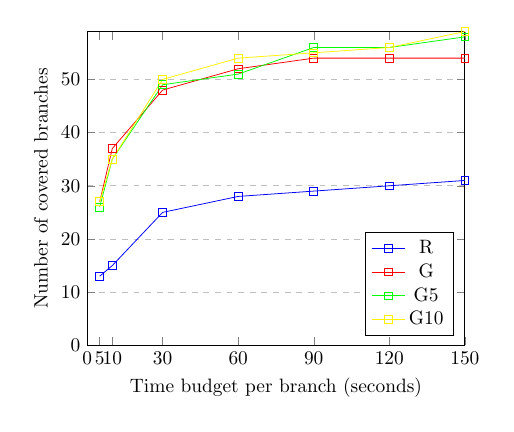
\begin{tikzpicture}[scale=0.7]
\begin{axis}[
    xlabel={Time budget per branch (seconds)},
    ylabel={Number of covered branches},
    xmin=0, xmax=150,
    ymin=0, ymax=59,
    xtick={0,5,10,30,60,90,120,150,180},
    ytick={0,10,20,30,40,50},
    legend pos=south east,
    ymajorgrids=true,
    grid style=dashed,
]
 
  \addplot[
    color=blue,
    mark=square,
  ] coordinates {
    (5,13) (10,15) (30,25) (60,28) (90,29) (120,30) (150,31)
  }; 
  \addplot[
    color=red,
    mark=square,
  ]  coordinates {
    (5,27) (10,37) (30,48) (60,52) (90,54) (120,54) (150,54)
  };
  \addplot[
    color=green,
    mark=square,
  ]   coordinates {
    (5,26) (10,35) (30,49) (60,51) (90,56) (120,56) (150,58)
  };
  \addplot[
    color=yellow,
    mark=square,
  ]   coordinates {
    (5,27) (10,35) (30,50) (60,54) (90,55) (120,56) (150,59)
  };
    \legend{R,G,G5,G10}
 
\end{axis}
\end{tikzpicture}
\caption{Progress of the branch coverage given fix time budget per branch}
\end{figure}

\subsection{Limitations}
\label{sub.sec.eval.limit}

Our framework imposes certain constraints on the structure of JS programs:
\begin{itemize}
\item no inter-procedural function calls
\item no recursion  
\end{itemize}


%% --------------------------------------------------------------------
\section{Related Work}
\label{sec:related.work}
%% --------------------------------------------------------------------

\subsection{Search-Based Test Case Generation}
\label{sub.sec.search.based}

\cite{wegener2001evolutionary} evolutionary test generation for structural coverage.

\cite{tonella2004evolutionary} evolutionary testing of classes

\cite{wappler2005using} evolutionary testing of object-oriented software.

\cite{wappler2006evolutionary} uses strongly-typed genetic programming and deals with the runtime exceptions.

\cite{lakhotia2007multi} multi-objective search-based test data generation 

\cite{cao2009search} multi-path search-based test data generation

\cite{awedikian2009mc} MC/DC test input generation 

\cite{shahbazi2016black} generation of string test data

\cite{fraser2012mutation} mutation-driven generation of unit tests and oracles

\cite{havrikov2014xmlmate} XMLMate: evolutionary XML test generation.

\cite{mcminn2004search} seminal survey of search-based test data generation techniques.

\cite{mcminn2011search} recent overview of search-based testing.

\cite{mairhofer2011search} search-based testing for dynamic languages (Ruby)

\cite{baars2011symbolic} combines dynamic analysis with symbolic information to improve search-based testing

\cite{alshahwan2011automated} automated web application testing using search based software techniques.

\cite{ma2015grt} guided random testing

\cite{mao2016sapienz} Multi-objective automated testing for Android application

\subsection{Static and Dynamic Analysis of JavaScript}
\label{sub.sec.js.static.anal}

Static analysis is a powerful technique commonly used as solid alternative for program testing. In fact both techniques can benefit from one another. For such weakly typed and dynamic languages as JavaScript employing static analysis to infer types can be an invaluable source of information to identify potential bugs or even guarantee their absence. Jensen et al.~\cite{tajs2009} presented such an analysis for JavaScript using abstract interpretation. In the follow-up work~\cite{dom2011} they extended the analysis with the abstractions to reason about HTML DOM and browser API. Given step let the authors to carry static analysis at the level of complete web application (JavaScript + HTML).
\cite{jquery2014}


ACTARUS is a static taint analysis of JS\cite{guarnieri2011saving}.

Jalangi is dynamic analysis framework for JavaScript \cite{sen2013jalangi}.

Dynamic type inconsistency analysis (implemented on top Jalangi) for JavaScript\cite{pradel2015typedevil}.

Salable dynamic analysis framework for JS based on shadow executions~\cite{create.citation}.

Information-flow security for JS~\cite{hedin2012information}.

\subsection{Whole Web Application Testing}
\label{sub.sec.web.app.test}

Artemis~\cite{artemis2011} is a feedback-directed random testing tool for JavaScript web application. It discoverers new tests by generating sequences of executable events and monitoring they effect on the state of the application. \cite{ail2013}

Testing of AJAX application by means of crawling of the application to infer state-flow graph~\cite{mesbah2012crawling} ATUSA ~\cite{mesbah2012invariant}

Learning DOM invariants from multiple executions of the application~\cite{pattabiraman2010dodom}.

Measuring test adequacy for web application based on the DOM state coverage~\cite{mirzaaghaei2014dom}.

Combining human written test cases with the automatically generated once by crawling in order to extend test coverage~\cite{milani2014leveraging}.

DOM-aware JavaScript code completion~\cite{bajaj2014dompletion}. 

\subsection{Formal Techniques}
\label{sub.sec.formal}

Modeling and reasoning about DOM events~\cite{lerner2012modeling}.

\subsection{JavaScript Unit Testing}
\label{sub.sec.js.unit.test}

Generating fixture for JavaScript unit tests by means of concolic execution~\cite{amin:ase15}. Inference of UI oracles to complement JS unit tests~\cite{icst16}.

JS unit test generation by means of symbolic execution~\cite{tanida2014automatic}.

Flycatcher~\cite{deautomatic}

\subsection{Misc JavaScript Testing Techniques}
\label{sub.sec.misc.test.tech}

Discover patterns from bug fixes and imposing them as potential bugs in the future~\cite{quinn:fse16}. 

\section{Conclusion}
\label{sec:concl}
1 page.

\bibliographystyle{ACM-Reference-Format}
\bibliography{icse2018.bib} 


\end{document}
